% -*- Mode:TeX -*-

%% IMPORTANT: The official thesis specifications are available at:
%%            http://libraries.mit.edu/archives/thesis-specs/
%%
%%            Please verify your thesis' formatting and copyright
%%            assignment before submission. If you notice any
%%            discrepancies between these templates and the 
%%            MIT Libraries' specs, please let us know
%%            by e-mailing thesis@mit.edu

%% The documentclass options along with the pagestyle can be used to generate
%% a technical report, a draft copy, or a regular thesis. You may need to
%% re-specify the pagestyle after you \include cover.tex. For more
%% information, see the first few lines of mitthesis.cls. 

%\documentclass[12pt,vi,twoside]{mitthesis}
%%
%%  If you want your thesis copyright to you instead of MIT, use the
%%  ``vi'' option, as above.
%%
\documentclass[12pt,vi,twoside,leftblank]{mitthesis}
%%
%% If you want blank pages before new chapters to be labelled ``This
%% Page Intentionally Left Blank'', use the ``leftblank'' option, as
%% above. 

%\documentclass[12pt,twoside]{mitthesis}
\usepackage{lgrind}

%% for figures
\usepackage[utf8]{inputenc}
\usepackage{graphicx}
\graphicspath{{templates/images/}}

%% for tables
\usepackage[normalem]{ulem}
\useunder{\uline}{\ul}{}

%% These have been added at the request of the MIT Libraries, because
%% some PDF conversions mess up the ligatures.  -LB, 1/22/2014
\usepackage{cmap}
\usepackage[T1]{fontenc}
\pagestyle{plain}

%% for List of Acronyms
\usepackage[acronym,toc]{glossaries}
\makenoidxglossaries

%% stylize hyperlinks
\usepackage{hyperref}
\usepackage{xcolor}
\hypersetup{
    colorlinks = true,
    linkcolor = blue,
    citecolor = blue
}

%% APA citations
\usepackage{apacite}
\usepackage{natbib}

\usepackage{xparse}
\ExplSyntaxOn

\makeatletter
\NewDocumentCommand{\multicitep}{m}
 {
  \NAT@open
  \mjb_multicitep:n { #1 }
  \NAT@close
 }
\makeatother

\seq_new:N \l_mjb_multicite_in_seq
\seq_new:N \l_mjb_multicite_out_seq
\seq_new:N \l_mjb_cite_seq

\cs_new_protected:Npn \mjb_multicitep:n #1
 {
  \seq_set_split:Nnn \l_mjb_multicite_in_seq { ; } { #1 }
  \seq_clear:N \l_mjb_multicite_out_seq
  \seq_map_inline:Nn \l_mjb_multicite_in_seq
   {
    \mjb_cite_process:n { ##1 }
   }
  \seq_use:Nn \l_mjb_multicite_out_seq { ;~ }
 }

\cs_new_protected:Npn \mjb_cite_process:n #1
 {
  \seq_set_split:Nnn \l_mjb_cite_seq { , } { #1 }
  \int_compare:nTF { \seq_count:N \l_mjb_cite_seq == 1 }
   {
    \seq_put_right:Nn \l_mjb_multicite_out_seq
     { \citeauthor{#1},~\citeyear{#1} }
   }
   {
    \seq_put_right:Nx \l_mjb_multicite_out_seq
     {
      \exp_not:N \citeauthor{\seq_item:Nn \l_mjb_cite_seq { 1 }},~
      \exp_not:N \citeyear{\seq_item:Nn \l_mjb_cite_seq { 1 }},~
      \seq_item:Nn \l_mjb_cite_seq { 2 }
     }
   }
 }
\ExplSyntaxOff

%% This bit allows you to either specify only the files which you wish to
%% process, or `all' to process all files which you \include.
%% Krishna Sethuraman (1990).

%\typein [\files]{Enter file names to process, (chap1,chap2 ...), or `all' to process all files:}
\def\all{all}
\ifx\files\all \typeout{Including all files.} \else %\typeout{Including only \files.} \includeonly{\files} \fi

%% define list of acronyms
\newacronym{aeo}{AEO}{Annual Energy Outlook}
\newacronym{ann}{ANN}{Artificial Neural Network}
\newacronym{aoi}{AOI}{Area of Interest}
\newacronym{auc}{AUC}{Area Under the ROC Curve}
\newacronym{bht}{BHT}{Bottom Hole Temperature}
\newacronym{br}{BR}{Basin and Range}
\newacronym{bnn}{BNN}{Bayesian Neural Network}
\newacronym{cnn}{CNN}{Convolutional Neural Network}
\newacronym{cp}{CP}{Colorado Plateau}
\newacronym{cv}{CV}{Cross Validation}
\newacronym{dem}{DEM}{Digital Elevation Model}
\newacronym{doe}{DOE}{United States Department of Energy}
\newacronym{dt}{DT}{Decision Tree}
\newacronym{egs}{EGS}{Enhanced Geothermal Systems}
\newacronym{eia}{EIA}{United States Energy Information Administration}
\newacronym{ebk}{EBK}{Empirical Bayes Kriging}
\newacronym{ep}{E\&P}{Exploration and Production}
\newacronym{fcn}{FCN}{Fully Connected Network}
\newacronym{fn}{FN}{False Negative}
\newacronym{fp}{FP}{False Positive}
\newacronym{fpr}{FPR}{False Positive Rate}
\newacronym{gdh}{GDH}{Geothermal District Heating}
\newacronym{ghg}{GHG}{Greenhouse Gas}
\newacronym{gis}{GIS}{Geographic Information System}
\newacronym{gto}{GTO}{Geothermal Technologies Office}
\newacronym{iea}{IEA}{International Energy Agency}
\newacronym{ieo}{IEO}{International Energy Outlook}
\newacronym{irena}{IRENA}{International Renewable Energy Agency}
\newacronym{kde}{KDE}{Kernel Density Estimation}
\newacronym{kgra}{KGRA}{Known Geothermal Resource Area}
\newacronym{kwh}{kW$\cdot$h}{Kilowatt-Hour}
\newacronym{lanl}{LANL}{Los Alamos National Laboratory}
\newacronym{lcoe}{LCOE}{Levelized Cost of Electricity}
\newacronym{lr}{LR}{Logistic Regression}
\newacronym{ma}{Ma}{Million Years Ago}
\newacronym{mdvf}{MDVF}{Mogollon-Datil Volcanic Field}
\newacronym{mwh}{MW$\cdot$h}{Megawatt-Hour}
\newacronym{nan}{NaN}{Not a Number}
\newacronym{nfegs}{NF-EGS}{Near Field EGS}
\newacronym{ngds}{NGDS}{National Geothermal Data System}
\newacronym{nmfk}{NMFk}{Non-negative Matrix Factorization \& k-means Clustering}
\newacronym{nm}{NM}{New Mexico}
\newacronym{nn}{NN}{Neural Network}
\newacronym{nrel}{NREL}{National Renewable Energy Laboratory}
\newacronym{ovo}{OvO}{One versus One}
\newacronym{ovr}{OvR}{One versus Rest}
\newacronym{opec}{OPEC}{Organization of the Petroleum Exporting Countries}
\newacronym{pca}{PCA}{Principle Component Analysis}
\newacronym{pfa}{PFA}{Play Fairway Analysis}
\newacronym{relu}{ReLU}{Rectified Linear Unit}
\newacronym{rfe}{RFE}{Recursive Feature Elimination}
\newacronym{rgr}{RGR}{Rio Grande Rift}
\newacronym{roc}{ROC}{Receiver Operating Characteristic}
\newacronym{shap}{SHAP}{Shapley Additive Explanation}
\newacronym{sigt}{SiGT}{Silica Geothermometer Temperature}
\newacronym{tn}{TN}{True Negative}
\newacronym{tp}{TP}{True Positive}
\newacronym{tpr}{TPR}{True Positive Rate}
\newacronym{usgs}{USGS}{United States Geological Survey}
\newacronym{voi}{VOI}{Value of Information}
\newacronym{xgb}{XGB}{XGBoost}

%% zotero integration
%\addbibresource{zotero}

\begin{document}

% -*-latex-*-
% 
% For questions, comments, concerns or complaints:
% thesis@mit.edu
% 
%
% $Log: cover.tex,v $
% Revision 1.9  2019/08/06 14:18:15  cmalin
% Replaced sample content with non-specific text.
%
% Revision 1.8  2008/05/13 15:02:15  jdreed
% Degree month is June, not May.  Added note about prevdegrees.
% Arthur Smith's title updated
%
% Revision 1.7  2001/02/08 18:53:16  boojum
% changed some \newpages to \cleardoublepages
%
% Revision 1.6  1999/10/21 14:49:31  boojum
% changed comment referring to documentstyle
%
% Revision 1.5  1999/10/21 14:39:04  boojum
% *** empty log message ***
%
% Revision 1.4  1997/04/18  17:54:10  othomas
% added page numbers on abstract and cover, and made 1 abstract
% page the default rather than 2.  (anne hunter tells me this
% is the new institute standard.)
%
% Revision 1.4  1997/04/18  17:54:10  othomas
% added page numbers on abstract and cover, and made 1 abstract
% page the default rather than 2.  (anne hunter tells me this
% is the new institute standard.)
%
% Revision 1.3  93/05/17  17:06:29  starflt
% Added acknowledgements section (suggested by tompalka)
% 
% Revision 1.2  92/04/22  13:13:13  epeisach
% Fixes for 1991 course 6 requirements
% Phrase "and to grant others the right to do so" has been added to 
% permission clause
% Second copy of abstract is not counted as separate pages so numbering works
% out
% 
% Revision 1.1  92/04/22  13:08:20  epeisach

% NOTE:
% These templates make an effort to conform to the MIT Thesis specifications,
% however the specifications can change. We recommend that you verify the
% layout of your title page with your thesis advisor and/or the MIT 
% Libraries before printing your final copy.
%\title{Machine Learning and Cost Analysis for Risk Management in Geothermal Exploration and Production}
\title{Geothermal Risk Mitigation Strategies for the Energy Transition}

\author{Robert Chadwick Holmes}
% If you wish to list your previous degrees on the cover page, use the 
% previous degrees command:
%       \prevdegrees{A.A., Harvard University (1985)}
% You can use the \\ command to list multiple previous degrees
%       \prevdegrees{B.S., University of California (1978) \\
%                    S.M., Massachusetts Institute of Technology (1981)}
\department{System Design and Management Program}

% If the thesis is for two degrees simultaneously, list them both
% separated by \and like this:
% \degree{Doctor of Philosophy \and Master of Science}
\degree{Master of Science in Engineering and Management}

% As of the 2007-08 academic year, valid degree months are September, 
% February, or June.  The default is June.
\degreemonth{September}
\degreeyear{2021}
\thesisdate{August 6, 2021}

%% By default, the thesis will be copyrighted to MIT.  If you need to copyright
%% the thesis to yourself, just specify the `vi' documentclass option.  If for
%% some reason you want to exactly specify the copyright notice text, you can
%% use the \copyrightnoticetext command.  
%\copyrightnoticetext{\copyright IBM, 1990.  Do not open till Xmas.}

% If there is more than one supervisor, use the \supervisor command
% once for each.
\supervisor{Aim\'e Fournier}{Research Scientist, Earth and Planetary Sciences}
\supervisor{Bryan R. Moser}{Academic Director, System Design and Management}

% This is the department committee chairman, not the thesis committee
% chairman.  You should replace this with your Department's Committee
% Chairman.
\chairman{Joan Rubin}{Executive Director, System Design and Management}

% Make the titlepage based on the above information.  If you need
% something special and can't use the standard form, you can specify
% the exact text of the titlepage yourself.  Put it in a titlepage
% environment and leave blank lines where you want vertical space.
% The spaces will be adjusted to fill the entire page.  The dotted
% lines for the signatures are made with the \signature command.
\maketitle

% The abstractpage environment sets up everything on the page except
% the text itself.  The title and other header material are put at the
% top of the page, and the supervisors are listed at the bottom.  A
% new page is begun both before and after.  Of course, an abstract may
% be more than one page itself.  If you need more control over the
% format of the page, you can use the abstract environment, which puts
% the word "Abstract" at the beginning and single spaces its text.

%% You can either \input (*not* \include) your abstract file, or you can put
%% the text of the abstract directly between the \begin{abstractpage} and
%% \end{abstractpage} commands.

% First copy: start a new page, and save the page number.
\cleardoublepage
% Uncomment the next line if you do NOT want a page number on your
% abstract and acknowledgments pages.
% \pagestyle{empty}
\setcounter{savepage}{\thepage}
\begin{abstractpage}
% $Log: abstract.tex,v $
% Revision 1.1  93/05/14  14:56:25  starflt
% Initial revision
% 
% Revision 1.1  90/05/04  10:41:01  lwvanels
% Initial revision
% 
%
%% The text of your abstract and nothing else (other than comments) goes here.
%% It will be single-spaced and the rest of the text that is supposed to go on
%% the abstract page will be generated by the abstractpage environment.  This
%% file should be \input (not \include 'd) from cover.tex.
%Geothermal provides a continuous, low greenhouse-gas emissions source of energy with enormous potential in the United States, both singularly or as part of a renewable energy portfolio. Although a small contributor to the current national energy grid, geothermal capture for generating electricity dates back nearly a century for natural hydrothermal systems. More recently, technologies at various readiness levels give the promise of geothermal access using enhanced geothermal systems (EGS), which provide engineered solutions for subsurface fluid circulation to tap into thermal reservoirs in a wider variety of locations. Nevertheless, the risk of high costs associated with exploration and production remain a hurdle to broader adoption of geothermal as part of a diverse commercial energy mix.

%In this thesis, risk-mitigation strategies for geothermal exploration and production target two separate aspects of the system lifecycle. The first considers how data collected for interrelated earth systems can indicate geothermal potential at the play and prospect scale. Analytical workflows integrating geologic and geophysical data are used to estimate the subsurface geothermal gradient, with quantitative uncertainty estimates associated with the data inputs, the modeling approach, and the size of the solution space. These uncertainty estimates provide a measure of risk, as well as decision tools for investments in additional data-gathering activities before the first well is drilled. The second focus looks at flexibility in engineering design with real options for expanding an existing power facility with geothermal. Specifically, key uncertainties are defined and integrated into a cost-modeling approach that uses decision rules to define an ensemble of possible outcomes. Tailoring the model and decision rules to the potential field and location of interest allows for a rapid but thorough test of project feasibility and the selection of build-out alternatives that limit downside risk and capture upside potential. In total, the learnings from these investigations provide insights into how geothermal can be a commercially viable, low-carbon option as energy companies navigate the ongoing energy transition.
Geothermal provides a continuous, low-emissions source of energy with enormous potential in the United States, both singularly or as part of a broader energy mix. Although a small contributor to the current national energy grid, geothermal electricity generation dates back nearly a century for natural hydrothermal systems. More recently, enhanced geothermal systems (EGS) promise a broader reach with engineered solutions for extracting subsurface heat from a wider variety of locations. The potential synergy between the oil \& gas and geothermal offers an opportunity for building a lower-carbon energy portfolio that requires compatible skills and expertise. Nevertheless, the risks involved at multiple stages of the field lifecycle remain a hurdle to adoption of geothermal.

In this thesis, risk-mitigation strategies for geothermal target two phases of the lifecycle: exploration and production. The first strategy uses a diverse set of measurements spanning multiple interrelated earth systems to collectively determine geothermal potential at the play scale. Analytical workflows integrate geologic, geochemical, and geophysical data to estimate subsurface geothermal gradient, with quantitative uncertainty estimates associated with the measurements, the models, and the solution space. These uncertainty estimates provide a measure of risk, as well as decision tools for investments in additional data-gathering activities before the first well is drilled. The second strategy applies flexibility in engineering design to a hypothetical EGS expansion of an existing power facility. Specifically, key uncertainties are integrated into a cost model with operational decision rules to create an ensemble of possible outcomes. Tailoring the model and decision rules to a particular facility concept allows for a rapid feasibility testing and optimization of project actions that limit downside risk while capturing upside potential. Both of these strategies use uncertainty characterization to reduce the threat of high-consequence geothermal risks. And by including them in a broader risk management approach, oil \& gas companies can make data-driven decisions on investing in geothermal during the energy transition.
\end{abstractpage}

% Additional copy: start a new page, and reset the page number.  This way,
% the second copy of the abstract is not counted as separate pages.
% Uncomment the next 6 lines if you need two copies of the abstract
% page.
% \setcounter{page}{\thesavepage}
% \begin{abstractpage}
% % $Log: abstract.tex,v $
% Revision 1.1  93/05/14  14:56:25  starflt
% Initial revision
% 
% Revision 1.1  90/05/04  10:41:01  lwvanels
% Initial revision
% 
%
%% The text of your abstract and nothing else (other than comments) goes here.
%% It will be single-spaced and the rest of the text that is supposed to go on
%% the abstract page will be generated by the abstractpage environment.  This
%% file should be \input (not \include 'd) from cover.tex.
%Geothermal provides a continuous, low greenhouse-gas emissions source of energy with enormous potential in the United States, both singularly or as part of a renewable energy portfolio. Although a small contributor to the current national energy grid, geothermal capture for generating electricity dates back nearly a century for natural hydrothermal systems. More recently, technologies at various readiness levels give the promise of geothermal access using enhanced geothermal systems (EGS), which provide engineered solutions for subsurface fluid circulation to tap into thermal reservoirs in a wider variety of locations. Nevertheless, the risk of high costs associated with exploration and production remain a hurdle to broader adoption of geothermal as part of a diverse commercial energy mix.

%In this thesis, risk-mitigation strategies for geothermal exploration and production target two separate aspects of the system lifecycle. The first considers how data collected for interrelated earth systems can indicate geothermal potential at the play and prospect scale. Analytical workflows integrating geologic and geophysical data are used to estimate the subsurface geothermal gradient, with quantitative uncertainty estimates associated with the data inputs, the modeling approach, and the size of the solution space. These uncertainty estimates provide a measure of risk, as well as decision tools for investments in additional data-gathering activities before the first well is drilled. The second focus looks at flexibility in engineering design with real options for expanding an existing power facility with geothermal. Specifically, key uncertainties are defined and integrated into a cost-modeling approach that uses decision rules to define an ensemble of possible outcomes. Tailoring the model and decision rules to the potential field and location of interest allows for a rapid but thorough test of project feasibility and the selection of build-out alternatives that limit downside risk and capture upside potential. In total, the learnings from these investigations provide insights into how geothermal can be a commercially viable, low-carbon option as energy companies navigate the ongoing energy transition.
Geothermal provides a continuous, low-emissions source of energy with enormous potential in the United States, both singularly or as part of a broader energy mix. Although a small contributor to the current national energy grid, geothermal electricity generation dates back nearly a century for natural hydrothermal systems. More recently, enhanced geothermal systems (EGS) promise a broader reach with engineered solutions for extracting subsurface heat from a wider variety of locations. The potential synergy between the oil \& gas and geothermal offers an opportunity for building a lower-carbon energy portfolio that requires compatible skills and expertise. Nevertheless, the risks involved at multiple stages of the field lifecycle remain a hurdle to adoption of geothermal.

In this thesis, risk-mitigation strategies for geothermal target two phases of the lifecycle: exploration and production. The first strategy uses a diverse set of measurements spanning multiple interrelated earth systems to collectively determine geothermal potential at the play scale. Analytical workflows integrate geologic, geochemical, and geophysical data to estimate subsurface geothermal gradient, with quantitative uncertainty estimates associated with the measurements, the models, and the solution space. These uncertainty estimates provide a measure of risk, as well as decision tools for investments in additional data-gathering activities before the first well is drilled. The second strategy applies flexibility in engineering design to a hypothetical EGS expansion of an existing power facility. Specifically, key uncertainties are integrated into a cost model with operational decision rules to create an ensemble of possible outcomes. Tailoring the model and decision rules to a particular facility concept allows for a rapid feasibility testing and optimization of project actions that limit downside risk while capturing upside potential. Both of these strategies use uncertainty characterization to reduce the threat of high-consequence geothermal risks. And by including them in a broader risk management approach, oil \& gas companies can make data-driven decisions on investing in geothermal during the energy transition.
% \end{abstractpage}

\cleardoublepage

\section*{Acknowledgments}

The past year will be long remembered for the impact a global pandemic had on society at large. This thesis is a product of that time. Those mentioned below played a significant role in keeping things on track in spite of the many months of mask wearing; hand sanitizing; regular virus testing; quarantining; remote classes, meetings, and connection-building; and eventual vaccination. Some I have even met in person, although not all. That is all part of the legacy of this most unusual and memorable year.

[Advisor]

[SDM - Readers, important individuals]

[ERL - NST Group]

[Chevron - Company]

[Chevron cohorts]

[Family]

%%%%%%%%%%%%%%%%%%%%%%%%%%%%%%%%%%%%%%%%%%%%%%%%%%%%%%%%%%%%%%%%%%%%%%
% -*-latex-*-

% Some departments (e.g. 5) require an additional signature page.  See
% signature.tex for more information and uncomment the following line if
% applicable.
% % -*- Mode:TeX -*-
%
% Some departments (e.g. Chemistry) require an additional cover page
% with signatures of the thesis committee.  Please check with your
% thesis advisor or other appropriate person to determine if such a 
% page is required for your thesis.  
%
% If you choose not to use the "titlepage" environment, a \newpage
% commands, and several \vspace{\fill} commands may be necessary to
% achieve the required spacing.  The \signature command is defined in
% the "mitthesis" class
%
% The following sample appears courtesy of Ben Kaduk <kaduk@mit.edu> and
% was used in his June 2012 doctoral thesis in Chemistry. 

\begin{titlepage}
\begin{large}
This doctoral thesis has been examined by a Committee of the Department
of Chemistry as follows:

\signature{Professor Jianshu Cao}{Chairman, Thesis Committee \\
   Professor of Chemistry}

\signature{Professor Troy Van Voorhis}{Thesis Supervisor \\
   Associate Professor of Chemistry}

\signature{Professor Robert W. Field}{Member, Thesis Committee \\
   Haslam and Dewey Professor of Chemistry}
\end{large}
\end{titlepage}


\pagestyle{plain}
  % -*- Mode:TeX -*-
%% This file simply contains the commands that actually generate the table of
%% contents and lists of figures and tables.  You can omit any or all of
%% these files by simply taking out the appropriate command.  For more
%% information on these files, see appendix C.3.3 of the LaTeX manual. 
\tableofcontents
\newpage
\listoffigures
\newpage
\listoftables


\printnoidxglossary[type=acronym, title=List of Acronyms, toctitle=List of Acronyms]
\printacronyms
\cleardoublepage
\chapter{Introduction}\label{ch1:intro}
The pursuit of energy has shaped the history of mankind from its very beginning. And while the image of ancient humans huddled around fires for warmth, protection, and meal preparation is an archetype of our ancestral past, modern human needs remain much the same. Lighting to extend day into night, heating and cooling for residential comfort, cooking of the food we eat, access to the advanced technologies of our time --- these all require energy from one source or another. Choices abound, from animal and plant-based fuels, to buried hydrocarbon resources, to alternatives like solar, wind, hydro, nuclear, and geothermal. The balance and utilization of these resources can shape societal growth on the geopolitical stage and influence the very future of the habitable Earth.

This thesis examines risk-mitigation strategies to help advance the role of one source, geothermal, in addressing ever-growing energy needs in a viable way. This chapter reflects on the extent of those needs and the conditions that may uniquely support an increased focus on geothermal as part of a commercial energy portfolio in the near-term. Opportunities and challenges associated with geothermal also lay the foundation for research questions motivating the remainder of this body of work.

\section{Energy Trends}\label{ch1:trends}
The \acrlong{eia} (\acrshort{eia}) publishes annual forecasts on U.S.\ energy generation and consumption in the \acrlong{aeo} (\acrshort{aeo}) report. Based on the 2020 reference case, the AEO model predicts a 70\% increase in U.S.\ energy usage by 2050, driven primarily by the industrial and power sectors \citep{eia_annual_2021}. Electricity generation also grows by a third, largely due to renewables and natural gas as coal, nuclear, and oil experience reductions (Figure \ref{fig:eia_2021_projections}). These predictions are offered with the caveat of greater uncertainty in the wake of the COVID-19 pandemic, although the EIA suggests a return to normal will occur by 2025 and broader, decadal trends will remain unchanged \citep{eia_annual_2021}. International forecasts show similar growth in consumption and production, but traditional sources of energy like coal and natural gas also increase in capacity to meet the needs of India, China, and other rapidly developing nations \citep{eia_international_2020}. 
 
\begin{figure}[htp]
\centering
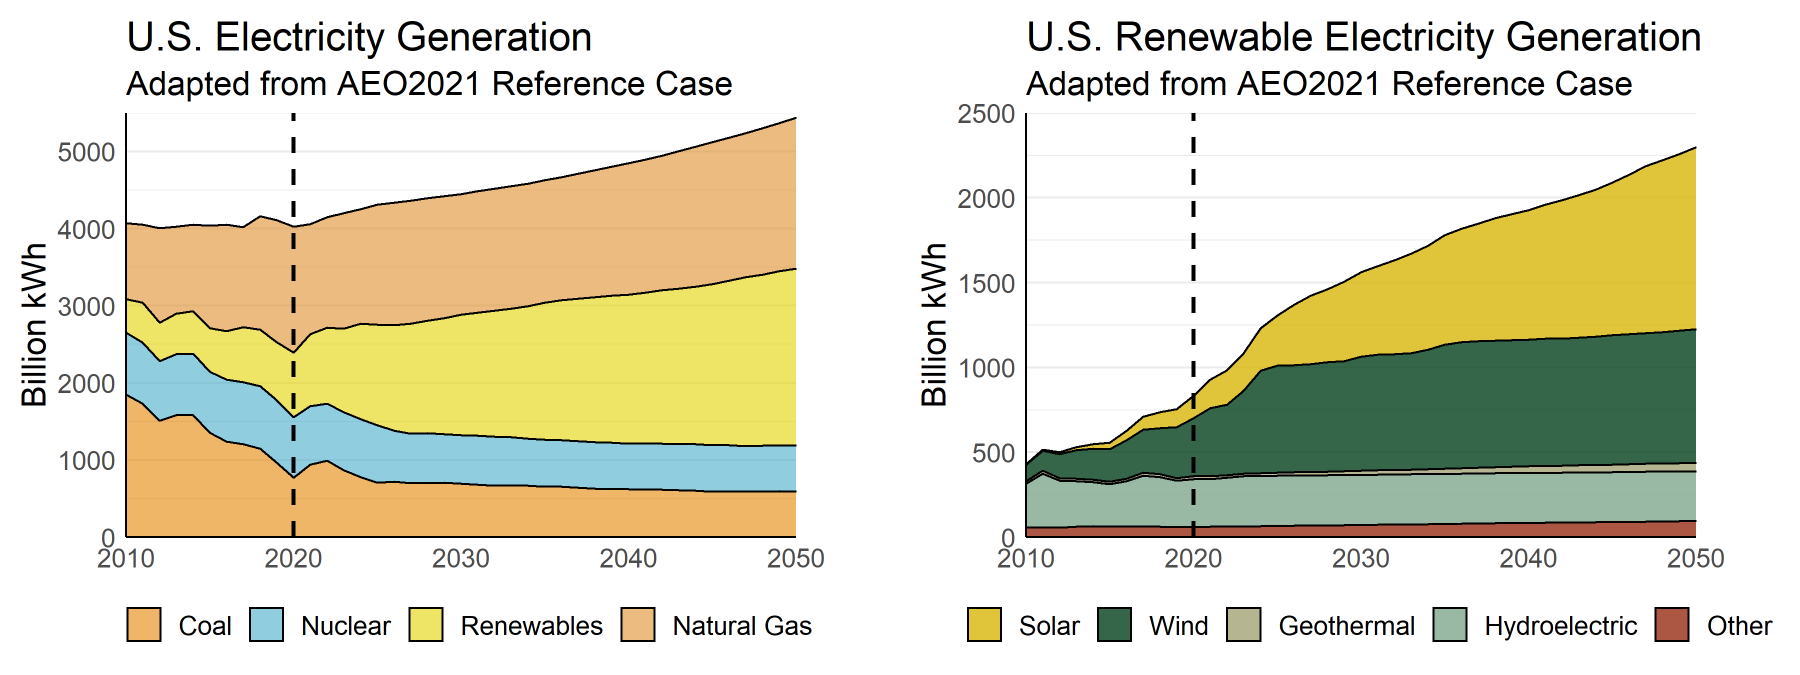
\includegraphics[width=\textwidth]{templates/images/Figure-EIA_projections.png}
\caption[U.S.\ EIA projections based on the AEO2021 reference case]{U.S.\ EIA projections of (Left) U.S.\ electricity generation by fuel source and (Right) individual contributions by renewables based on the AEO2021 reference case \protect\citep{eia_annual_2021}. Vertical dashed line marks where historical records end and projections begin.}
\label{fig:eia_2021_projections}
\end{figure}

Lazard Asset Management breaks renewables down by \acrlong{lcoe} (\acrshort{lcoe}) in U.S.\ dollars/MWh, where \acrshort{lcoe} is the estimated lifetime average net cost per unit energy of an electricity-generating plant. In their 2020 analysis, intermittent energy sources like wind and utility-scale solar are already cost-competitive with fossil fuel-derived sources (Figure \ref{fig:lazard_lcoe}) \citep{lazard_lazards_2020}. Geothermal, an “always on” source of power, ranges from \$59-\$101/MWh LCOE, making it second-tier in cost-competitiveness but comparable to community and rooftop solar installations \citep{lazard_lazards_2020}. Overall, the transition away from fossil fuel super-dominance is in progress, and the demand for energy in support of population growth and country development will remain an industry driver over the next 30 years.
 
\begin{figure}[htp]
\centering
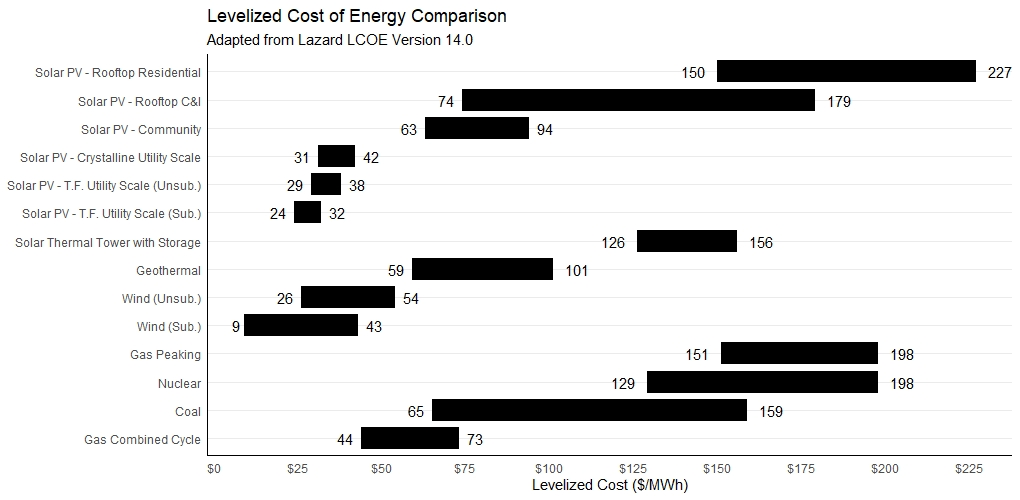
\includegraphics[width=\textwidth]{templates/images/Figure-Lazard_LCOE_recreated.jpeg}
\caption[Lazard Levelized Cost of Energy 2021 projections]{Cost comparison between different energy sources based on Lazard Asset Management LCOE analysis. C\&I: Commercial \& Industrial, T.F.: Thin Film, Unsub.: Unsubsidized, Sub.: Subsidized. For specific assumptions and caveats related to the analysis, see \protect\citep{lazard_lazards_2020}.}
\label{fig:lazard_lcoe}
\end{figure}

\section{Upstream Commercial Pressures}\label{ch1:upstream}
Businesses focused on exploration and production of oil \& gas face a growing list of pressures influencing future corporate strategy. On one hand, the increase in energy consumption predicted by the AEO and IEO supports a steady increase in production to meet global demand; however, geopolitical tensions, state-ownership of oil companies, and breakthrough technologies create a volatile landscape unforgiving of an unsophisticated production approach. In just the past 15 years, major downturns in oil prices were triggered by a mixture of factors: the financial crisis, tied to banking practices and housing market instability in 2008 \citep{singh_2007-2008_2021}; increased production from U.S.\ unconventional plays and supply decisions from the Organization of the Petroleum Exporting Countries (OPEC) in 2014 \citep{lioudis_what_2021}; and a price war between Russia and Saudi Arabia coinciding with a global pandemic in 2020 \citep{blessing_what_2021}. Additional uncertainty comes from National Oil Companies (NOCs) that control the majority of the world’s petroleum reserves, production, and rights for exploration and development. NOCs operate under different business drivers than International Oil Companies (IOCs), with ramifications on the stability of IOC investments and access to reserves as seen in Russia and Venezuela \citep{bremmer_long_2010,pirog_role_2007}. Meanwhile, disruptive technologies like precise directional drilling and efficient hydraulic fracturing have freed access to previously cost-prohibitive reserves, changing the balance of power as countries like the U.S.\ and China become less reliant on foreign hydrocarbon imports \citep{shuen_dynamic_2014}.

Layered on top of these macroeconomic influences are unexpected events that have enormous impact on energy production and distribution operations. The 2020 outbreak of COVID-19 acted as an accelerator on longer-term trends of digital transformation and decarbonization in the oil \& gas industry. In the wake of a 25\% decrease in global demand, companies responded with massive layoffs and restructuring, a heightened focus on digitalization, and portfolio rationalizations that include shale write-downs and asset divestments \citep{deloitte_2021_2020}. Also, extreme weather events consistent with global warming predictions are shining a critical spotlight on how energy is managed now and in the future. Blackouts, water outages, and surge pricing on electricity impacted millions of Texans in February 2021 when a winter storm brought record cold temperatures, exposing systematic weaknesses in energy infrastructure and generator preparedness for low-probability but feasible working conditions \citep{harc_winter_2021,lazard_lazards_2020}. And additional threats loom in the cyberworld as malicious hacking activities have rippling social and financial implications. One such attack on Colonial Pipeline, which handles almost 50\% of the liquid fuels supplied to the U.S.\ East Coast, led to gasoline shortages, price spikes, chemical factory shut-downs, and worldwide news coverage until the nearly \$5 million in ransom was paid in May 2021 \citep{sanger_pipeline_2021}.

\section{Net Zero Ambitions}\label{ch1:netzero}
The 2015 Paris climate agreement set a target of $<2^\circ$C on the rise in global temperatures above the pre-industrial average (i.e., the period from 1850-1900) to prevent the most extreme impacts of climate change \citep{unfccc_paris_2015}. The more commonly-ascribed $1.5^\circ$C target may be unachievable given current trajectories, and international calls to action are focusing on reducing anthropogenic carbon dioxide emissions to ``net zero'' as quickly as possible \citep{ipcc_global_2018}. Greater public awareness about the environmental impacts of global warming and alignment with these targets is putting pressure on the energy industry to revise their traditional business models. Beginning in 2020, top-tier oil and gas companies started issuing press releases outlining energy transition targets for 2025, 2030, 2050, and beyond \citep{bp_international_2020,chevron_chevron_2021,conocophillips_conocophillips_2020,equinor_equinor_2020,exxonmobil_exxonmobil_2021,shell_responsible_2020,shell_shell_2021,total_total_2020,total_2020_2021}. The proposed strategies vary but generally focus on (i) reducing company stake in fossil-fuel exploration and production activities, (ii) setting a net zero target applicable to emissions from operations, product carbon intensity, and carbon offsets, and (iii) dedicating investments in low- and no-carbon energy alternatives to replace hydrocarbons. Nevertheless, the pressure to do more, faster reached a new peak in May 2021 when a court decision in The Netherlands and approved shareholder proposals for two U.S.\ majors demanded an accelerated push toward emissions reductions and low-carbon energy options \citep{mcwilliams_investors_2021}.

\section{Geothermal Energy}\label{ch1:geothermal}
Several factors must be met for an energy source to be considered a viable and sustainable alternative to the carbon-based fuels (coal, natural gas, oil) that currently meet much of the world’s energy needs. \citeauthor{glassley_geothermal_2015} outlines a succinct set of criteria for such an energy resource: i) self-replenishment, ii) adequate abundance to meet energy demands, iii) low- to no-greenhouse gas emissions, and iv) cost competitiveness compared to accessible alternatives (\citeyear[p.\ 7]{glassley_geothermal_2015}). The first criterion precisely characterizes renewable sources of energy like solar, gravitational, and geothermal. Solar energy includes both direct (sunlight) and indirect (wind, waves, water cycle) resources \citep{hohmeyer_ipcc_2008}. Gravitational energy drives the tides and supports energy-storage solutions like pumped-storage hydropower \citep{eere_pumped-storage_2021,hohmeyer_ipcc_2008}. And geothermal energy is derived from accretionary heat and natural decay of radioactive isotopes within the Earth \citep{hohmeyer_ipcc_2008}. Table \ref{tab:renewableflux} specifically addresses criterion ii; the annual abundances of most renewable sources exceed energy demand, with geothermal scaling several orders of magnitude greater in annual flux/demand than other options \citep{hohmeyer_ipcc_2008}. Geothermal also meets the third criterion by providing a no-carbon source of energy that could support net zero aspirations when used in place of fossil fuels. The fourth criterion is less clear-cut. Geothermal costs depend strictly on use case, but as noted in Section \ref{ch1:trends}, LCOE analysis currently ranks geothermal below wind and solar in the list of renewable options \citep{lazard_lazards_2020}. Does this make geothermal non-viable as an alternative? Perhaps no, as geothermal comes with several unique opportunities and benefits.

\begin{table}[h!]
\centering
\begin{tabular}{|l|l|l|}
\hline
\textbf{Renewable Source} & \textbf{Annual flux (EJ/yr)} & \textbf{Annual Flux/Demand*} \\ \hline
Solar      & 3,900,000   & 8,700  \\ \hline
Wind       & 6,000       & 13     \\ \hline
Hydro      & 149         & 0.33   \\ \hline
Bioenergy  & 2,900       & 6.5    \\ \hline
Ocean      & 7,400       & 17     \\ \hline
Geothermal & 140,000,000 & 31,000 \\ \hline
\end{tabular}
\caption[Annual renewable energy fluxes]{Annual renewable energy fluxes, adapted from Table 1 of \protect\citep{hohmeyer_ipcc_2008}. The (*) indicates flux/demand ratio is derived from global demand estimates.}
\label{tab:renewableflux}
\end{table}

Most fundamentally, geothermal energy offers a reliable, nearly inexhaustible resource accessible anywhere around the world. Unlike wind and solar, which depend on favorable locations and vary with both season and time of day, geothermal is ubiquitous and continuous. Furthermore, it can provide baseload power for regional electrical grids without the additional need of assistive energy-storage technology \citep{tester_future_2006}. Based on history, one might assume geothermal only works under conventional hydrothermal conditions, e.g., near active volcanoes (e.g., Iceland, Indonesia) or within major rift zones (e.g., East African Rift). However, additional opportunities lie in low-temperature direct-use geothermal for heating and cooling of buildings, industrial processing, agricultural activities, and manufacturing \citep[p.\ 9]{glassley_geothermal_2015}. And technology supporting Enhanced Geothermal Systems (EGS) provides access to subsurface heat in areas without hydrothermal conditions \citep{tester_future_2006}. Natural radioactive decay takes place throughout the Earth’s crust, contributing to the global rise in temperature with depth known as the geothermal gradient \citep[p.\ 279]{fowler_solid_2005}. Where conditions permit access to suitable depths, there is the potential for geothermal energy capture.

For all its benefits, the use of geothermal energy comes with a set of challenges that are unique among renewable energy options. Many mirror issues faced by oil \& gas producers, like failures in drilling equipment or borehole integrity. Others include risk of low resource quality, poor reservoir productivity, unexpected structural and stratigraphic complexity, and undesirable fluid chemistry \citep{beckers_low-temperature_2016, hadi_resource_2010}. The similarities extend into unconventionals/EGS, where hydrofracturing risks comprise inadequate permeable rock volume within the stimulated fracture zone, short-circuiting of fluid flow between injection and productions wells, fluid losses within the subsurface, and induced seismic activity \citep{jelacic_evaluation_2008,pan_establishment_2019}. As in oil \& gas projects, some of these risks can be mitigated through appropriate subsurface characterization, others from high-resolution reservoir and fracture modeling. Collectively, the overlap in operational challenges and the skill sets required to tackle them defines a unique compatibility between oil \& gas and geothermal. Knowledge transfer between the two domains could directly benefit geothermal operations and risk-mitigation strategies \citep{petty_synergies_2009}. And investing in geothermal assets could take upstream companies a step closer to meeting net-zero commitments while retaining and utilizing existing talent.

One of the most significant uncertainties for geothermal is cost. The scope of an LCOE assessment considers all costs in a geothermal project, from early exploration, through development drilling and power plant construction, to operations and maintenance over a 25- to 30-year lifetime \citep{beckers_introducing_2013, entingh_volume_2006, tester_economic_1990}. Studies show drilling of exploration, appraisal, injection, and production wells can account for 60-75\% of the total EGS project expenses \citep{lukawski_uncertainty_2016, petty_synergies_2009}. New technologies being developed may help address future drilling costs \citep{lowry_geovision_2017,nrel_2020_2020}. However, substantial project savings could also be achieved through better characterization prior to drilling the first exploration well; increasing the probability of well success without multi-million dollar well failures would certainly reduce LCOE. In addition, choices in the design of the geothermal power plant may also have significant cost implications over the life of a geothermal field. Lessons can be learned from power plants built to design specifications incompatible with actual production conditions \citep[e.g.,][]{manente_hybrid_2011}. Improving the economics of geothermal start with recognizing uncertainties in the system and using those uncertainties to make better decisions on \textit{where to drill} and \textit{how to produce}. Providing the appropriate tools and methods to make these decisions could also help oil \& gas companies manage the risk of embracing lower-carbon energy production with geothermal as part of their energy mix.

\section{Research Questions}\label{ch1:researchqs}
Based on the above-mentioned opportunity to define methods that incorporate uncertainty characterization for risk management in geothermal exploration and production, this thesis will address the following research questions:

\begin{enumerate}
  \item Can geothermal exploration risk be mitigated by insights derived from readily-available data sources with little change in project cost? Can the data establish additional actions for further risk reduction before drilling a geothermal well? 
  \item How can characterization of present and future uncertainties influence the development and production strategy for geothermal facilities? In what ways will such an approach mitigate risk, if at all?
\end{enumerate}

\hfill\break
\section{Thesis Outline}\label{ch1:outline}
This thesis follows the flow shown in Figure \ref{fig:thesis_flow} and is structured as follows: 
\begin{figure}[!htp]
\onehalfspacing
\begin{minipage}[b]{0.5\textwidth}
\begin{itemize}
\item Chapter 2 provides relevant background material on geothermal systems, a literature review on geothermal exploration and cost modeling, and a primer on case study areas investigated in later chapters.
\item Chapters 3--4 describe the thesis data sources, data preparation strategies, and the chosen methods for favorability prediction with machine learning (Ch.\ 3) and cost modeling of geothermal project designs (Ch.\ 4).
\item Chapters 5--6 describe the machine learning model results (Ch.\ 5) and cost modeling results (Ch.\ 6).
\item Chapter 7 frames learnings from the previous chapters as risk mitigation actions in an overall risk management workflow.
\end{itemize}
\end{minipage} \hfill
\begin{minipage}[b]{0.47\textwidth}
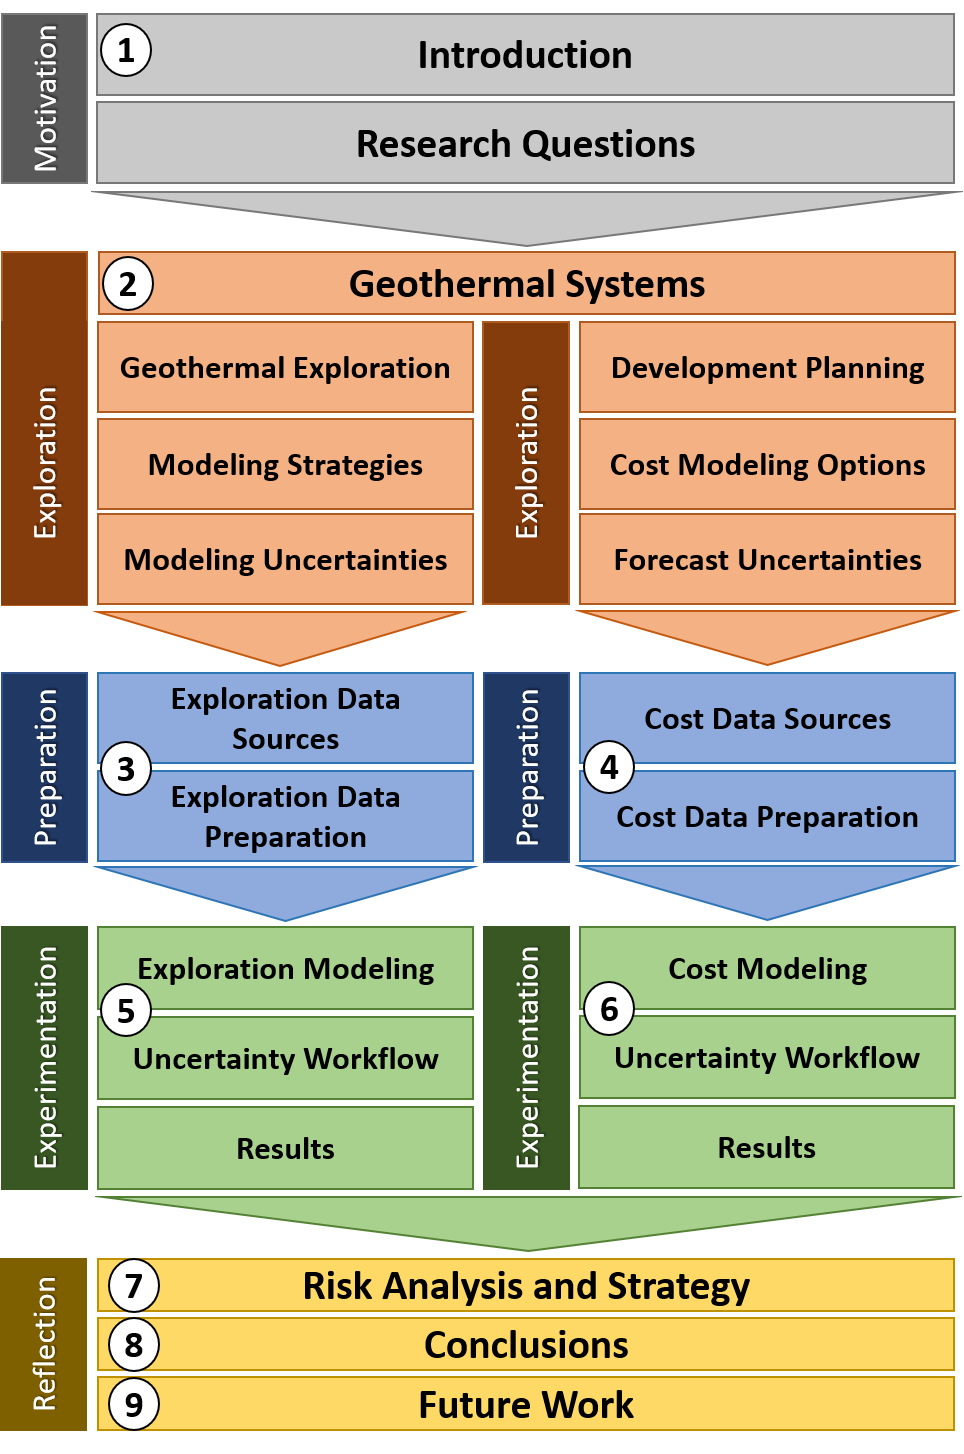
\includegraphics[scale=0.47]{Figure-ThesisWorkflow}
\caption[Thesis structure flow chart]{Flow chart of thesis structure. Chapter numbers are circled.}
\label{fig:thesis_flow}
\end{minipage}
\begin{itemize}
\item Chapters 8 and 9 conclude the thesis with a summary of thesis insights (Ch.\ 8) and a list of future work opportunities (Ch.\ 9).
\end{itemize}
\end{figure}
\chapter{Background}\label{ch2:background}

\section{Geothermal Systems}\label{ch2:geosys}
\subsection{Heat Origins}\label{ch2:heatorig}
\subsubsection{Accretion}\label{ch2:accrete}
The story of geothermal energy begins with the birth of planet Earth. Approximately 4.56 billion years ago \citep{allegre_age_1995, patterson_age_1956}, the Earth coalesced as a molten body heated by repeated impacts with objects in the early solar system like the planetesimal impact responsible for the formation of the Moon \citep{stevenson_origin_2014}. Over tens of millions of years, the Earth compacted, cooled, and differentiated, settling into the familiar layered structure of a solid inner core, liquid outer core, viscous mantle, and outermost brittle crust \citep[~p. 7]{press_understanding_2004}. The intense heat from that early accretionary history remains concentrated in the core, where temperatures - a matter of continued scientific inquiry - fall in the range of 6000±500 K \citep[~p. 372]{fowler_solid_2005}. Present day heat flux estimates for the whole Earth amount to 87 mW/m\textsuperscript{2}, \texttt{\char`\~}60\% of which flows through conductive and convective pathways from the deep interior to outermost crust \citep{stein_heat_1995}. Diffuse conductive heat transfer occurs everywhere across of the Earth’s surface, but heat flow concentrates along tectonic plate boundaries. In fact, the subduction-sourced volcanoes that ring the Pacific Ocean, divergent zones at the mid-ocean ridges and East African rift, and major strike-slip boundaries like the San Andreas fault zone all mark locations where focused heat anomalies are already being tapped by geothermal installations \citep[~p. 16]{dipippo_geothermal_2012}.
\subsubsection{Radioactive Decay}\label{ch2:radio}
The second major source of heat within the Earth is the decay of radioactive isotopes. Early radioactive heating included radioisotopes with short half-lives like Aluminum-26 and Hafnium-182, which are now no longer present \citep[~p. 16]{glassley_geothermal_2015}. Among the radioactive elements contributing the most to heating the crust today are uranium (U), thorium (Th), rubidium (Rb), and potassium (K) \citep[~p. 17]{glassley_geothermal_2015}. The decay of these and other elements accounts for 40\% of the crustal thermal budget \citep{stein_heat_1995}. But element abundances are not distributed uniformly throughout the crust. On average, continental crust, particularly the upper continental crust, has significantly higher concentrations of U, Th, and K radioactive elements compared to oceanic crust, and both types of crust are 1-2 orders of magnitude more enriched than the mantle \citep[~p. 276]{fowler_solid_2005}. This relationship holds for representative igneous rock types; granite generates more heat than basalt, and both out-produce ultramafic rocks like peridotites \citep[~p. 276]{fowler_solid_2005}.
\subsection{Heat Measurements}\label{ch2:heatmeas}
\subsubsection{Geothermal Gradient}\label{ch2:geotherm}
Average subsurface conditions show a steady increase in temperature with depth, commonly referred to as the geothermal gradient, sustained by the flow of original accretionary heat and generated radioactive heat. On average, the gradient for continental crust is \texttt{\char`\~}30\textdegree C/km \citep[~p. 209]{press_understanding_2004}. However, deviations from this value are common and reflect the complexity of the rock record in an area. The crust comprises a distinct set of layers, or strata, that vary in composition and rock type. Unlike the aforementioned igneous formations that can be relatively homogeneous, surface processes mix sediments from a variety of original source rocks, sometimes sorting them well and sometimes not, before they get deposited and indurated into sedimentary formations \citep[~p. 164-168]{press_understanding_2004}. Alteration from fluids, heat, and pressure can then modify the composition of these rocks, causing constituent minerals to change form and arrangement to create metamorphic rocks \citep[~p. 195-205]{press_understanding_2004}. The spatial and depth variations in these formations create subsurface compositional heterogeneity, directly reflected in rock properties. Thermal conductivity, specifically the ability to move deep-sourced heat to shallower depths, and radioactive element abundance, or the ability to generate additional heat in situ, can therefore vary in all directions in the subsurface. Thermal heterogeneity can be further compounded by anomalies created from salt movement \citep[~p. 164-168]{press_understanding_2004}, magmatic intrusions, or global tectonic processes. It therefore takes a good understanding of the geology and geologic history to determine the geothermal gradient of a region.
\subsubsection{Heat Flow}\label{ch2:heatflow}
Fundamentally, heat moves from hot to cold (Second Law of Thermodynamics) at a rate that linearly scales with the thermal gradient. Simple, one-dimensional thermal conduction can be characterized by the relationship \citep[~p. 270]{fowler_solid_2005}:
\begin{equation}\label{eq:conduction}
q = -k \frac{\nabla T}{x}
\end{equation}
where q is heat flux, or heat flow per unit time per unit area, with S.I. units of \(Wm^{-2}\). Heat flux depends on the gradient of temperature (T), the distance over which conduction takes place (x), and the thermal conductivity (k), that is, the ability of material to conduct heat. Different rock types have different values of k, e.g., sandstone varies from 1.60-2.10 \(W/m^\circ C\) while granite tends to be higher with values ranging from 1.73-3.98 \(W/m^\circ C\) \citep[~p. 30]{dipippo_geothermal_2012}. Feldspars and quartz exhibit significant (up to 3x) differences in k values. As the most abundant minerals in crustal rocks, their relative fractions will strongly influence the thermal conductivity of a formation \citep[~p. 22]{glassley_geothermal_2015}. Regardless, minerals tend to be relatively poor thermal conductors compared to other materials like aluminum (210 \(W/m^\circ C\)) and iron (73 \(W/m^\circ C\)), making conduction a slow method of crustal heat transmission \citep[~p. 23]{dipippo_geothermal_2012}.

Conduction dominates on local scales in the crust, while convection is the primary means of heat transfer on global, tectonic scales. Even in its two-dimensional form with no internal heat generation, the equation governing convection is much more complex than for conduction \citep[~p. 355]{lowrie_fundamentals_2007}:
\begin{equation}\label{eq:convection}
\frac{\partial T}{\partial t} = \left (\frac{k}{\rho * c_P}\right)\left (\frac{\partial ^2T}{\partial x^2}+\frac{\partial ^2T}{\partial z^2}\right)-u_x\frac{\partial T}{\partial x}-u_z\frac{\partial T}{\partial z}
\end{equation}
where \textbf{u} = \(( u_x, u_z)\) is the velocity of the fluid, \(\rho\) is the material density, and \(c_P\) is the specific heat, which defines the amount of heat necessary to raise 1 kg of that material by 1\(^\circ C\) Convention combines heat transfer from conduction with mass movement. Since the minerals are relatively poor conductors of heat, the combined effects of lower viscosity and thermal expansion – as seen near the core-mantle boundary – and gravitational forces that create buoyancy effects, all create the right conditions for convective flow, e.g. within the mantle \citep[~p. 25]{glassley_geothermal_2015}. Mantle convection is responsible for the high heat flow values observed at crustal plate boundaries like mid-ocean ridges, as well as intraplate diapiric hot spots underlying Hawaii, Yellowstone, and a number of other locations around the world.  Smaller-scale convection also takes place at subduction zones where the material from the down-diving plate melts at lower temperatures with the presence of water, migrates upwards, and forms volcanic arcs on the surface as observed in Japan, Indonesia, and the Pacific Northwest of the U.S. \citep[~p. 31-33]{press_understanding_2004} – all locations with geothermal potential.

Heat flow measurements capture the flux of heat through the Earth’s surface as a result of these and other complex processes taking place in the subsurface. In this respect, it serves as a simpler and more accessible metric for local or regional heat potential than the more sparsely-measured and less well-constrained geothermal gradient. Today, high-quality heat flow measurements can be obtained in marine conditions, on continental margins, on mid-ocean ridges, and from the multitude wells drilled by the oil \& gas industry, supporting the creation of large heat flow data sets like the New Global Heat Flow database \citep{lucazeau_analysis_2019}. As Figure \ref{fig:heatflow} shows, data from these collections can be gridded to create spectacular maps of heat flow variations around the world. These maps offer a good starting point for quickly targeting where the greatest geothermal potential exists at the regional or “play” scale, which can then be further refined through additional methods (see Section \ref{ch2:geoexp}).
\begin{figure}[h!]
\centering
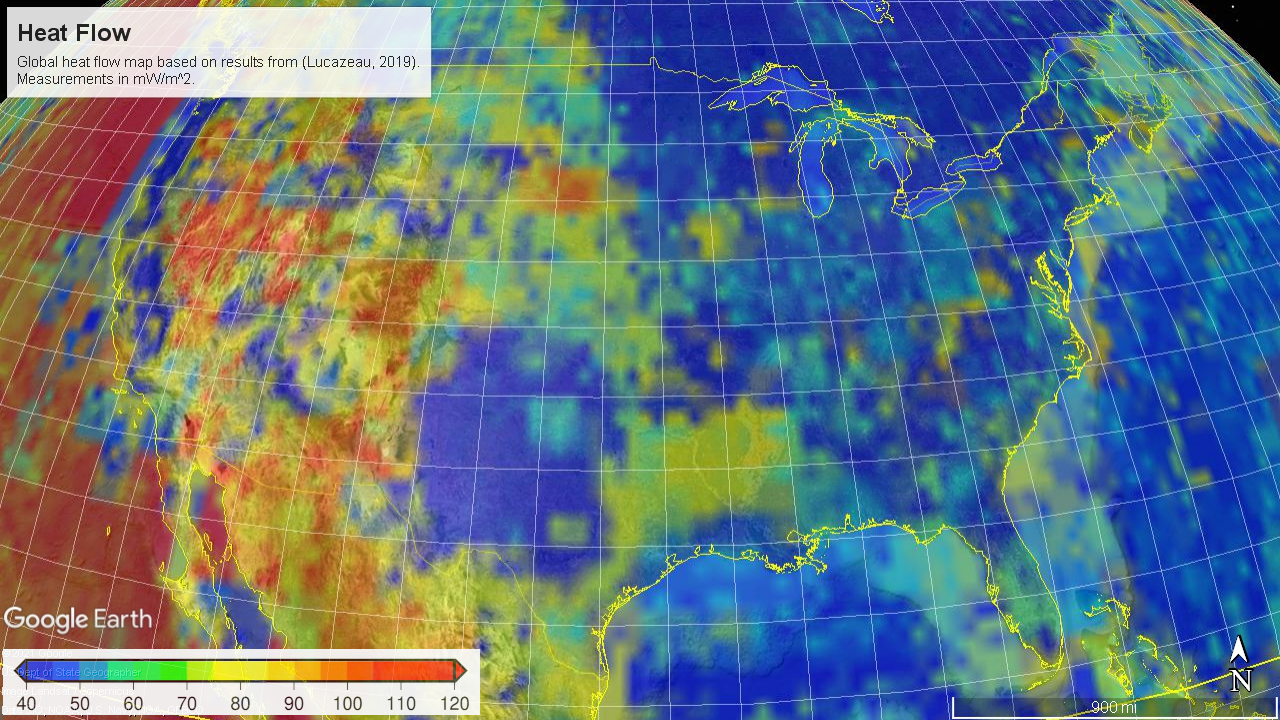
\includegraphics[scale=0.45]{Figure-HeatFlowMap}
\caption[Heat flow across the continental U.S.]{Heat flow estimates for the continental United States, plotted in Google Earth with data layer from \protect\citep{lucazeau_analysis_2019}}
\label{fig:heatflow}
\end{figure}
\subsection{System Fundamentals}\label{ch2:sysfund}
The conventional concept of a geothermal system consists of five key entities \citep[~p. 9]{dipippo_geothermal_2012}:
\renewcommand{\labelenumi}{\roman{enumi}}
\begin{enumerate}\label{list:sysreq}
   \item Heat source of significant size and temperature
   \item Permeability, typically in the form of a fracture network within crystalline rock
   \item Ample volume of working fluids, e.g. water from precipitation and drainage
   \item Impermeable sealing layer
   \item Consistent, reliable fluid recharge
\end{enumerate}

\subsubsection{Hydrothermal Systems}\label{ch2:hydro}
If naturally present, the combination of these five elements defines a hydrothermal system. As water percolates down, captures heat from the permeable thermal reservoir, and gets trapped beneath the sealing caprock, a small fraction of the resource can escape to the surface to produce distinctive geothermal manifestations like fumaroles, hot pools, geysers, mud pots, and discolored or altered rocks (Figures \ref{fig:lassen-geysers} and \ref{fig:lassen-mudpot}). These features are strong indicators of hydrothermal resources at depth.
\begin{figure}[h!]
\centering
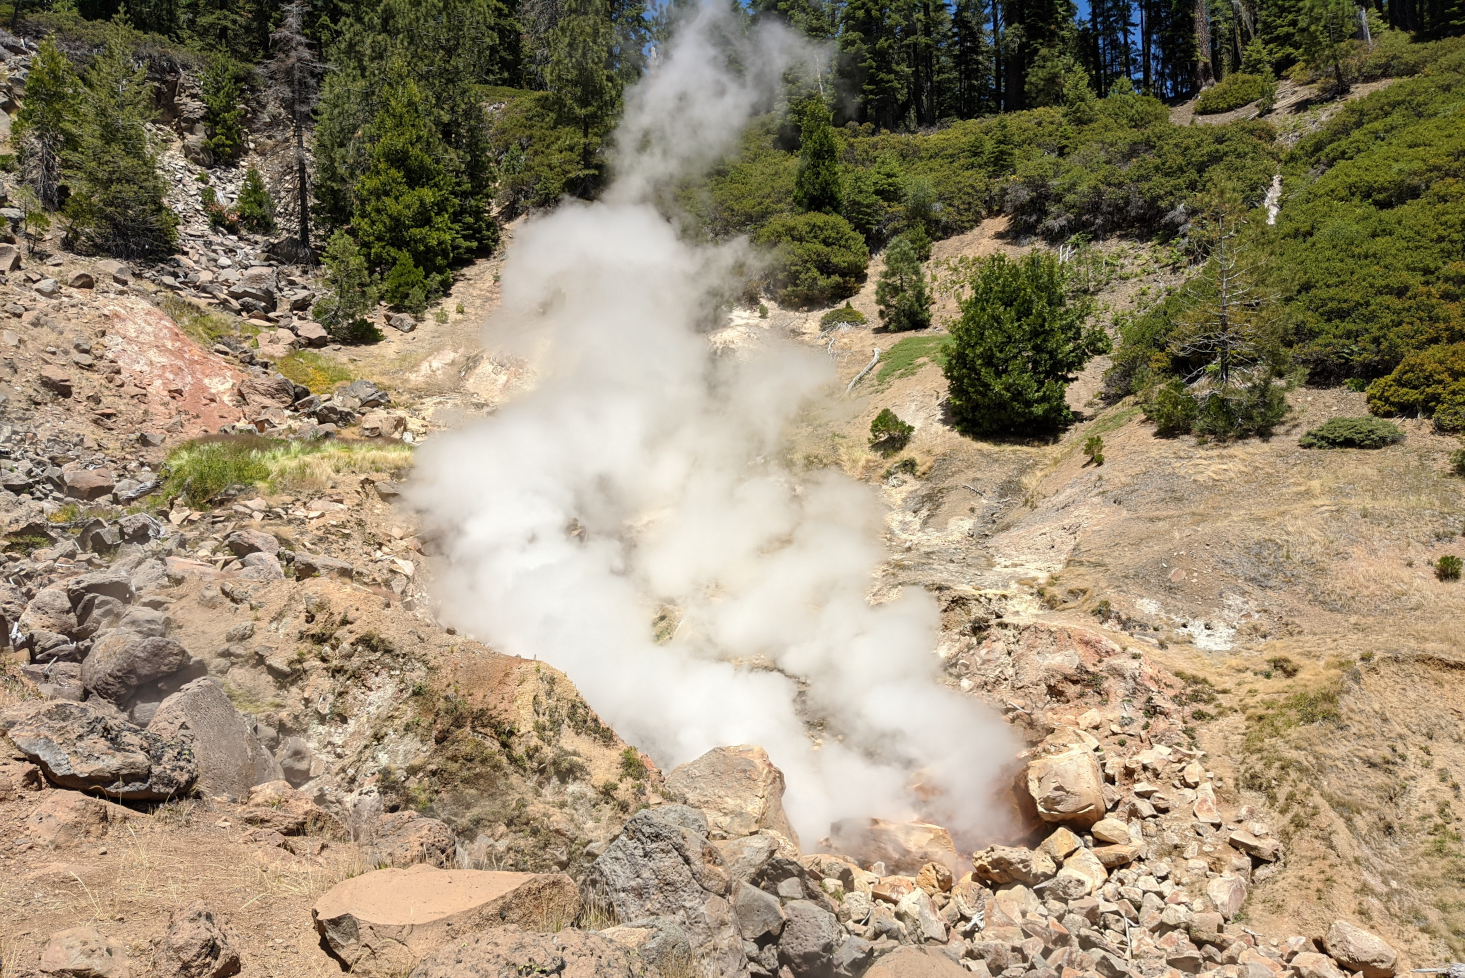
\includegraphics[scale=.84]{Figure-Lassen-geysers3}
\caption[Terminal Geyser, Lassen National Park]{Terminal Geyser, Lassen National Park, California. Photo credit: Author}
\label{fig:lassen-geysers}
\end{figure}
\begin{figure}[htbp]
\centering
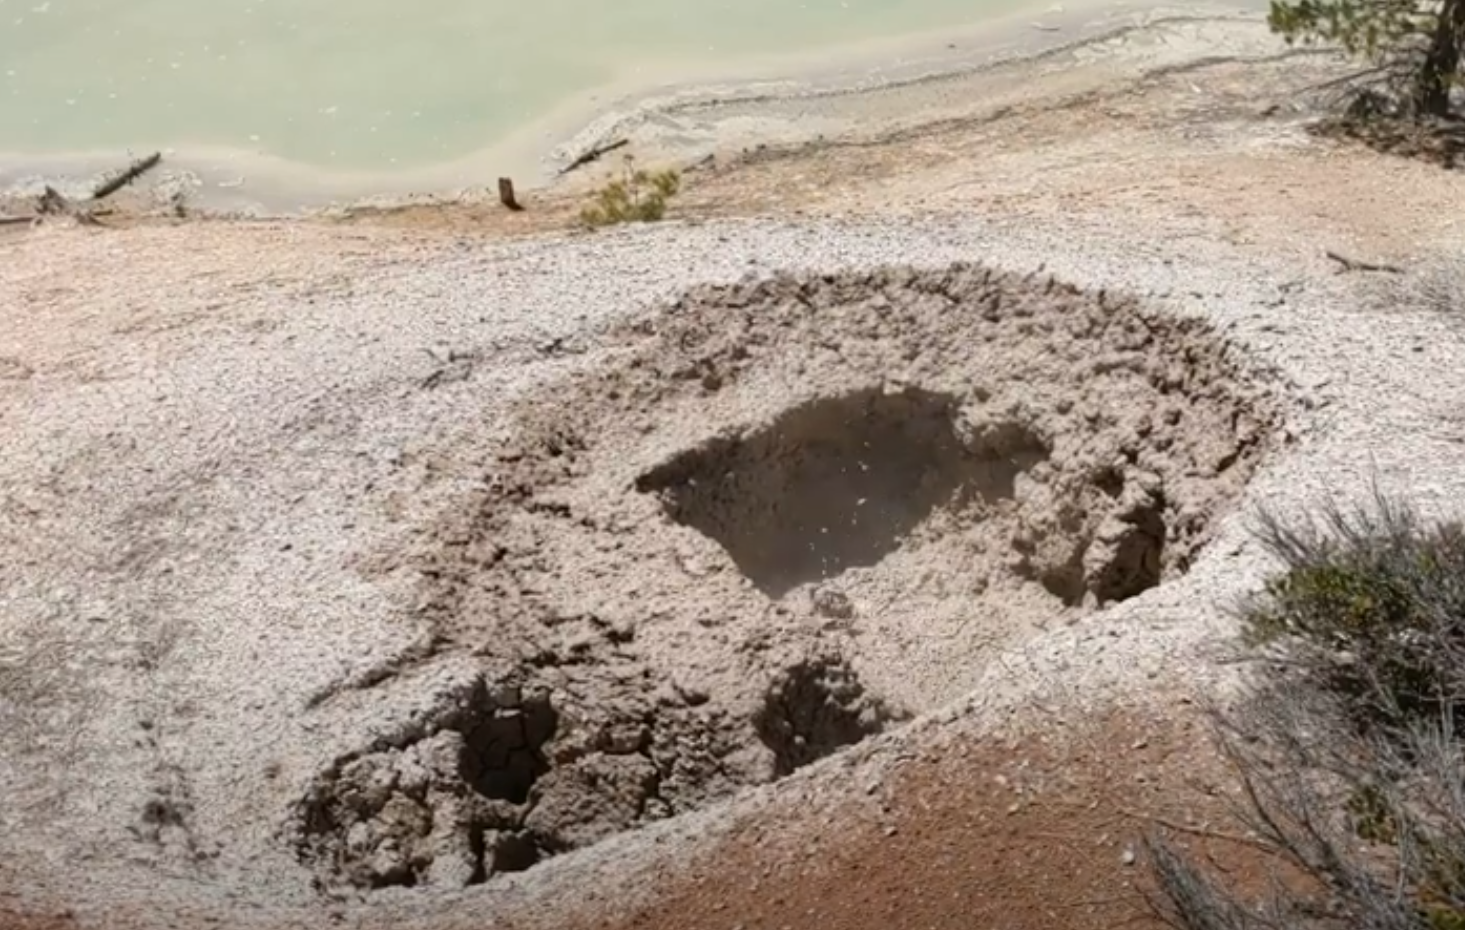
\includegraphics[scale=0.27]{Figure-Lassen-mudpot}
\caption[Mud pot, Lassen National Park]{Active mud pot and ground staining on the bank of Boiling Springs Lake, Lassen National Park, California. Photo credit: Author}
\label{fig:lassen-mudpot}
\end{figure}
The original geothermal systems exploited by mankind for millennia are hydrothermal systems. Artifacts show proto-Native American use of hydrothermal waters for cleaning and health restoration over 10,000 years ago \citep{doe_history_2021}. The importance of geothermal hot springs for Roman, Japanese, Chinese, and Ottoman baths is also well-established in the historical record \citep{lund_characteristics_2007}. Industrial use began in the 1800s with chemical extraction from geothermal steam, pools, and deposits in Larderello, Italy \citep[~p. 251]{dipippo_geothermal_2012}. \acrlong{gdh} (\acrshort{gdh}), or large-scale heating of residences and businesses using geothermal-produced fluids, was pioneered in Chaudes-Aigues, France in the 1300s and first introduced to the United States in 1892 with an installation in Boise, Idaho \citep{lund_characteristics_2007}.

These few examples capture some of the many potential opportunities for low-temperature (<90\(^\circ C\)) and medium-temperature (<150\(^\circ C\)) geothermal resource use, even beyond hydrothermal systems. GDH can help meet building and water temperature needs, and agriculture, textiles, paper, chemicals, and even the food industry can also benefit from access to low-temperature geothermal fluids \citep{doe_low_2021,liu_overview_2015}. Interest has led to funding from agencies like the \acrlong{gto} (\acrshort{gto}) within the \acrlong{doe} (\acrshort{doe}); a grant was recently awarded to Cornell University in support of piloting a deep direct-use project to provide baseload heating for the university campus supporting peak demand during cold upstate New York winter months  \citep{hamm_geothermal_2021,tester_integrating_2015}.

The topic of this thesis instead concerns the use of moderate- to high-temperature geothermal for power generation. The first example of geothermal power production came from Italian experiments in 1904, and the first commercial plant went online in Larderello, Italy in 1914 \citep[~p. 251]{dipippo_geothermal_2012}. Geothermal-generated electricity made its debut in the United States with the development of The Geysers field beginning in 1960 \citep{tester_future_2006}. Hydrothermal plants quickly appeared in New Zealand, Japan, Iceland, Indonesia, Kenya, Philippines and elsewhere throughout the 1970s-1980s, with continued growth through to present-day \citep{lund_characteristics_2007}. 2020 statistics from the \acrlong{irena} (\acrshort{irena}) place the United States as world leader in geothermal installed capacity (2587 MWe), followed by Indonesia (2131 MWe) and Philippines (1928 MWe) \citep{irena_country_2021} (Figure \ref{fig:irena-rank}). 

\begin{figure}[htbp]
\centering
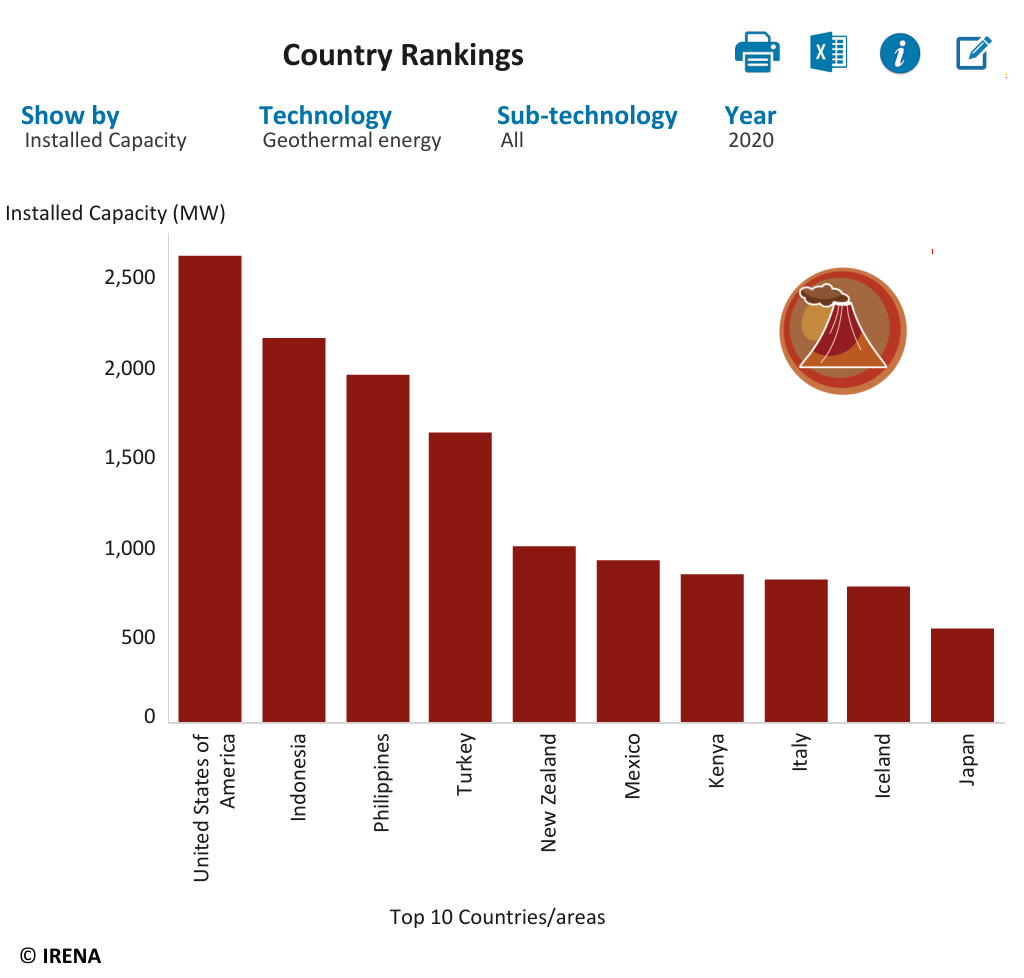
\includegraphics[scale=.45]{Figure-IRENA_Rankings}
\caption[Country rankings, installed geothermal capacity ]{Countries ranked by installed geothermal capacity, from \protect\citep{irena_country_2021}}
\label{fig:irena-rank}
\end{figure}

A comprehensive assessment of moderate and high-temperature \acrlong{kgra}s (\acrshort{kgra}s) by the \acrlong{usgs} (\acrshort{usgs}) determined the U.S. has conventional geothermal (hydrothermal) power generation potential of \texttt{\char`\~}9,000 MWe, and an additional \texttt{\char`\~}30,000 MWe potential exists in undiscovered resources \citep{williams_assessment_2008}. The recent DOE GeoVision study notes hydrothermal potential in Alaska and Hawaii alone are \texttt{\char`\~}8000 MWe due to their unique tectonic environments (Aleutian subduction zone and Hawaiian hot spot, respectively), and high-case model estimates for the continental U.S. forecast an installed capacity of \texttt{\char`\~}16.5 GW by 2050 for known and unknown hydrothermal resources \citep{augustine_geovision_2019,hamm_overview_2019}.

\subsubsection{Enhanced Geothermal Systems}\label{ch2:egs}
In some cases, the potential for a geothermal system exists even when one or more of the fundamental elements listed in Section \ref{ch2:sysfund} are missing. These unconventional geothermal systems, often referred to as \acrlong{egs} (\acrshort{egs}), contain a significant heat source but lack either the adequate permeability or sufficient rechargeable working fluids to meet the requirements of a hydrothermal system. A broader definition for EGS includes thermal production from sedimentary and crystalline tight rock, poorly-performing hydrothermal systems, co-production from oil \& gas operations, and even thermal recovery directly from magma \citep{tester_future_2006}. Focusing on the more common tight rock scenario, EGS systems work by artificially creating or improving reservoir permeability and ensuring sustained flow rates of fluids through the reservoir \citep[~p. 281]{glassley_geothermal_2015}. Fluids pumped down an injection well pass through a stimulated fracture network, heat up through direct contact with the thermal reservoir, and return to the surface via one or more producing wells to serve as inlet fluids for a power plant \textbf{MISSING FIGURE}. Reservoir stimulation generally involves hydraulic fracturing (hydro-fracking or just “fracking”) techniques to create pathways connecting injector-producer pairs. The associated technology and capabilities are thus well-aligned with unconventional oil \& gas operations \citep{petty_synergies_2009}. 

EGS can provide the bridge between geothermal use in niche hydrothermal environments and a more comprehensive adoption of geothermal energy for electricity generation across the United States. The sources of subsurface heat (see Section \ref{ch2:heatorig}) exist everywhere, so accessing a range of temperatures that could support power production relies on drilling deep enough and creating the artificial conditions necessary for heat capture. \acrlong{lanl} (\acrshort{lanl}) validated the EGS approach in crystalline rock at Fenton Hill beginning in 1974, soon after which feasibility studies were conducted in Japan, Germany, the U.K., and France \citep{breede_systematic_2013}. Among the most notable EGS projects that provided key lessons learned are The Geysers (U.S), Soultz-sous-Forêts (France), and Cooper Basin (Australia). The Geysers stands out as the largest geothermal power-generating complex in the world, providing \texttt{\char`\~}1,000 MWe for California even after 60 years of steam production \citep{jelacic_evaluation_2008,williams_assessment_2008}. Although drilling issues and public concern over induced seismicity halted efforts \citep{manish03_united_2009}, rock stimulation experiments in the Northwest Geysers proved distinct reservoirs can be developed adjacent to active hydrothermal operations \citep{pan_establishment_2019}. The Soultz project commenced in 1987 with one injector and two producers drilled to 5 km depth to support a 1.5 MW power plant built in 2007-2008 \citep[~p. 463]{dipippo_geothermal_2012}. In addition to many experimental lessons learned around drilling, hydrofracturing, chemical stimulation, scaling and corrosion, Soultz today supports both electricity production and direct-use district heating \citep{durst_overview_2013}. Cooper Basin, the largest EGS demonstration project in the world, showed great promise after a 6-year proof of concept phase \citep{stephens_assessing_2010}. However, the project halted in 2015 due poor stimulation results tied to an unrecognized fault, highlighting the importance of robust structural appraisal in assessing geothermal prospects \citep{holl_what_2015}. 

As the fate of these projects might suggest, the long-standing promise of EGS has not yet been fully realized. However, several active projects supported by the DOE and NREL (e.g. EDGE, FORGE, EGS Collab) are providing the insights necessary to mature subsurface models, drilling technologies, and stimulation methods for more widespread EGS adoption \citep{hamm_geothermal_2021}. And recent technology advances and partnerships involving start-ups Fervo Energy \citep{moss_google_2021,shieber_geothermal_2021}, Deep Earth Energy \citep{geoenergy_saskatchewan_2021}, Eavor Technologies \citep{ross_energy_2020}, and Climeon \citep{climeon_climeon_2021,geoenergy_baseload_2020} show there is a growing fervor to overcome the technology roadblocks currently holding EGS back. Projections show the size of the prize with success in EGS. Assuming a maximum cut-off depth of 7 km and a minimum reservoir temperature of 150\(^\circ C\), the EGS resource potential for electricity production in the continental United States might be at least \texttt{\char`\~}5,150 GWe, with an additional \texttt{\char`\~}1,500 MWe from NF-EGS \citep{augustine_geovision_2019}. To put this opportunity into context: the total utility-scale electricity generation capacity from \underline{all} sources in the United States was \texttt{\char`\~}1,200 GWe in 2019, over 4x less in magnitude \citep{eia_electric_2020}.

\section{Geothermal Exploration}\label{ch2:geoexp}
\subsection{Background}
Historically, the identification of geothermal resources primarily relied on surface expressions of hot fluids circulating at depth. Quite simply, if a bubbling hot spring or a geyser was present, you had a working hydrothermal system. Some of the first sites for geothermal power production, like Larderello and The Geysers, were unsurprisingly targeted because of their tell-tale surface characteristics \citep[~p. 111]{glassley_geothermal_2015}. However, this prospecting method only applies to fully-functioning hydrothermal systems, and not all such systems have surface manifestations if fluids remain trapped beneath a subsurface impermeable seal. These hidden or “blind” geothermal resources require more sophisticated exploration methods to identify and assess accurately.

\subsection{Regional Exploration}
Regional evaluation techniques classically relied on sparse borehole data, including water wells and oil \& gas wells, to map out the geothermal potential of the U.S. \citep{kehle_aapg_1970}. Successive efforts led to progressively more comprehensive collections of surface heat flow and borehole temperature measurements \citep{blackwell_temperature-at-depth_2011, blackwell_heat_1990, muffler_assessment_1979, sorey_low-temperature_1983, wisian_heat_1999}, now widely-available with other geothermal data through the DOE-funded National Geothermal Data System platform \citep{anderson_national_2013}. These efforts supported a better understanding of broad trends directly tied to tectonic provinces in the United States. Subduction and transform plate boundaries in the West, combined with extension in the Basin and Range, make this area of the U.S. more susceptible to high heat flow, high geothermal gradient, and greater potential for hydrothermal system activity \citep{mariner_low-temperature_1983}. Passive margins on the Atlantic and Gulf of Mexico sides make those regions less likely to host significant hydrothermal systems, although surveys have identified sedimentary basins with elevated heat flow in the south (Louisiana-Arkansas), central (Iowa-Illinois, Nebraska-South Dakota), and eastern (Appalachians) parts of the country \citep{blackwell_geothermal_1995, sorey_low-temperature_1983}.

\subsection{Sub-regional Exploration}
Continental maps provide a super-regional view of geothermal prospectivity, but further refinement is required to progress an exploration program. Specifically, the determination of regional plays and local prospects must come before deciding where and how to develop a geothermal field, e.g., for electricity generation. Characterization activities can be decomposed into defining the magnitude and extent of four earth subsystems: structural, stratigraphic, hydrologic, and thermal. The main types of surveys associated with each subsystem are listed in Table \ref{tab:surveytypes} and discussed briefly in the following section. Note that the various survey methods typically provide information on multiple subsystems. The associated non-uniqueness of subsurface interpretations based on these survey results highlights the need to integrate multiple lines of evidence for exploration activities. 

\begin{table}[!htp]
\begin{tabular}{ll}
\textbf{Structural}     & \textbf{}                                                \\ \hline
Aerial survey           & surface fault traces                                     \\
Earthquake records      & fault location, recency                                  \\
Geodetic survey         & active deformation or faulting                           \\
Geologic survey         & surface fault traces, fault recency                      \\
Gravity survey          & subsurface faults, plutons, salt                         \\
Resistivity survey      & fractured zones                                          \\
Satellite survey        & topography, structural patterns                          \\
Seismic surveys         & subsurface faults, folds, other structural features      \\
                        &                                                          \\
\textbf{Stratigraphic}  &                                                          \\ \hline
Geologic survey         & stratigraphic chart, seal and reservoir                  \\
Gravity survey          & density anomalies, stratigraphic variations              \\
Magnetic survey         & igneous formations, stratigraphy and reservoir           \\
Radiometric survey      & mineral abundances, source and reservoir                 \\
Resistivity survey      & thermal conductivity, lithology                          \\
Satellite survey        & distribution of outcrops and formations                  \\
Seismic survey          & stratigraphy and rock properties                         \\
                        &                                                          \\
\textbf{Hydrologic}     &                                                          \\ \hline
Earthquake records      & movement of magma or fluids                              \\
Geologic survey         & surface expressions (vents, geysers, deposits), drainage \\
Hydrologic survey       & fluid geochemistry, recharge and rate, water table       \\
Magnetic survey         & hydrothermal alteration                                  \\
Precipitation records   & water cycle inputs, recharge rate                        \\
Resistivity survey      & subsurface fluids or hydrothermal alteration             \\
Satellite survey        & surface drainage patterns, distribution of deposits      \\
Seismic survey          & presence and location of subsurface fluids               \\
                        &                                                          \\
\textbf{Thermal}        &                                                          \\ \hline
Aerial survey           & thermal anomalies in shallow subsurface (IR)             \\
Air Temperature records & near-surface thermal conditions                          \\
Geologic survey         & surface manifestations (dikes, vents, deposits)          \\
Gravity survey          & presence of high-T anomalies (e.g. magma)                \\
Hydrologic survey       & geothermometry, dominant geofluid liquid phase           \\
Radiometric survey      & radioactive heat generation                              \\
Resistivity survey      & thermal conductivity, temperature gradient               \\
Temperature survey      & heat flow, geothermal gradient                          
\end{tabular}
\caption{Data collection methods useful for characterizing and derisking Earth subsystems that influence geothermal favorability}
\label{tab:surveytypes}
\end{table}

\subsubsection{Geologic Data Collection}
Geologic field mapping in an area can provide crucial direct evidence supporting the presence of geothermal systems. Surface manifestations like geysers, vents, and mud pots may also be coincident with mappable mineralogic indicators of the subsurface chemistry and style of geothermal activity.  Volcanic-based geothermal systems tend to have acid-sulfate waters with hydrogen sulfide-rich brines that leave behind sulfur deposits \citep[~p. 123]{glassley_geothermal_2015}. Bicarbonate geothermal waters can produce distinctive travertine terraces or subaqueous tufa deposits, as well as a unique variety of K-spar called adularia \citep[~p. 125]{glassley_geothermal_2015}. And chloride geothermal fluids are known to precipitate sinter or geyserite deposits composed of opal or amorphous silica \citep[~p. 125]{glassley_geothermal_2015}. Elevated abundances of trace elements like boron and lithium typically occur in chloride brines compared to meteoric (derived from precipitation) waters, so their presence in mineral assemblages is also diagnostic \citep{bielicki_hydrogeolgic_2015, millot_multi-isotopic_2007}. Other valuable products of a geologic survey include maps of surface fault patterns to better constrain the structural history, as well as volcanic intrusive (dikes) and extrusive (flows) features for understanding the thermal history and potential deeper reservoir potential.

Direct geochemical analysis of springs, pools, and samples collected from wells provides additional insights into the hydrologic characteristics of an area. Water chemistry offers information on the dominant resource fluid phase (vapor vs. liquid), the temperature of the subsurface formations encountered by the fluids, and the nature of the original water source \citep[~p. 25]{dipippo_geothermal_2012}. The concentration or equilibria of different elements, e.g., quartz, chalcedony, sodium, potassium, and calcium, can be compared to empirically-derived trends for reservoir temperature estimates \citep[~p. 157]{glassley_geothermal_2015}. These geothermometry methods offer insights into the deep thermal regime, although uncertainty around fluid migration pathways disallows any clear designation of the exact location and depth of a thermal reservoir.

Field methods like water sampling and geologic mapping offer local insights that can be interpolated for a bigger picture understanding of an area, with the caveat that field data tend to be limited in both number and spatial distribution. Aerial and satellite surveys provide regionally extensive measurements without the spatial sampling bias implicit in field activities. High-resolution topography captured in \acrlong{dem} (\acrshort{dem}) and their gradient (slope) can reveal morphology patterns tied to surface water drainage and recharge potential for deeper geothermal systems. Other optical products provide additional information of value; infrared imagery captures thermal anomalies in the shallow subsurface, stereographic images emphasize fault offsets missed in the field, and hyperspectral imaging can discriminate between different mineral assemblages, including geothermally-sourced boron-rich accumulations \multicitep{dipippo_geothermal_2012, ~p. 22;glassley_geothermal_2015, ~p. 154-155}.

\subsubsection{Geophysical Data Collection}
Geophysical methods also offer regional data coverage while also providing insights into how subsurface characteristics vary with depth. Magnetic surveys detect the magnetic fields imprinted on rocks that contain susceptible minerals and have experienced appropriate thermal conditions \citep[~p. 248-249]{lowrie_fundamentals_2007}. Magnetic anomalies, calculated by removing the regional magnetic field and non-geologic signals, can indicate the presence of intrusive volcanic bodies or hydrothermally-altered formations \citep[~p. 146]{glassley_geothermal_2015}. Gravity surveys similarly consider variations in local values after applying a regional gravity removal and other corrections \citep[~p. 59-62]{lowrie_fundamentals_2007}. Gravity anomalies highlight differences in subsurface density, which may be diagnostic of mineral alteration from hydrothermal processes, the presence of fractures, or pore fluid changes (e.g., replacement of meteoric water with hydrocarbons, hydrothermal fluids, or steam) \citep[~p. 150]{glassley_geothermal_2015}. Resistivity surveys measure electrical resistivity (or its inverse, conductivity) within an instrumented area – a property sensitive to fluids in rock pores or fractures and some variations in mineralogy, i.e., within alteration zones \citep[~p. 147]{glassley_geothermal_2015}. However, poor resolution beyond shallow (~1 km) depths strongly limits the reach of classic resistivity studies. Magnetotellurics (MT), measurements of currents induced by natural electromagnetic waves originating in the ionosphere, can extend conductivity insights much deeper, even into the upper mantle \citep[~p. 225]{lowrie_fundamentals_2007}. And seismic surveys, which measure acoustic wave propagation in the subsurface, can be processed and modeled to image stratigraphy, faults, fluids, and rock properties to a range of depths. Seismic refraction data can constrain whole crustal thickness \citep[e.g.][]{holmes_oceanic_2009}, with implications on heat flow, while seismic reflection data could define the thickness and extent of a geothermal reservoir and trapping geometry \citep[e.g.][]{cappetti_new_2005}.

\subsection{Strategies}
\subsubsection{Joint Inversion}

As powerful as geophysical methods are at remotely detecting earth properties, each method represents an inherently underconstrained problem. Complex mathematical routines can invert data collected by aerial survey (e.g., gravity, magnetics) or through surface acquisition techniques (resistivity, MT, seismic) to create 2D or 3D subsurface models. Still, unlike highly precise medical imaging technologies like Magnetic Resonance Imaging (MRI) that completely surround the target, geophysical techniques have a limited top-down view of the earth and must contend with noisy environments. Solutions to geophysical problems thus tend to be non-unique, and uncertainty increases with depth. Joint approaches to mathematical inversion for subsurface models address this ambiguity by constraining solutions to match the observations from multiple geophysical methods at once \citep{vozoff_joint_1975}. The complexity of a joint inverse problem applied to geothermal rapidly grows as more data sets are incorporated, particularly when the different data are sensitive to different earth properties \citep{moorkamp_framework_2011}. In addition, geothermal model results can meaningfully differ depending on the selected mathematical treatment used to generate solutions \citep{rosenkjaer_comparison_2015}. One alternative approach avoids the mathematical and computational demands by combining data semi-quantitatively, either by visually correlating individual model results or by cascading constraints from one geophysical model to the next to generate an integrated solution \citep{jousset_hengill_2011, lichoro_joint_2019}. Absent a tightly-coupled formulation of the relationship between all data inputs, the weighted influence of each data source must be chosen by the analyst, which can be a significant source of uncertainty.

\subsubsection{Play Fairway Analysis}

Regional or play scale exploration methods adapted from oil \& gas companies include geospatial risk assessments known as \acrlong{pfa} (\acrshort{pfa}). Conceptually, PFA breaks risk down into the constituent elements of a successful hydrocarbon play: reservoir, source, and seal \citep{fraser_regional_2010,nash_adaptation_2015}, and sometimes structure or trap \citep{doust_exploration_2010}. Maps are generated for each element based on any available data, including literature reviews, point data like wells or field sampling, and modeling results. Taking the collective evidence (or lack thereof) as input, subject matter experts provide a perception of chance as a probability, and statistical approaches combine the different probability maps into a cumulative favorability map and calculations of yet-to-find resource volumes \citep{lottaroli_evaluating_2018}. The Geothermal Technologies Office recently supported a number of projects focused on applying PFA techniques to identify geothermal plays across the United States, including blind and EGS geothermal systems \citep{eeri_play_2014}. Each study developed its own methodology for defining the primary geothermal play risk factors, quantifying uncertainty, and generating a final favorability map \citep{faulds_discovering_2019, jordan_low_2016, nash_phase_2017, wannamaker_structurally_2016}. Final numerical favorability scores were defined by a combination of risk elements, most often heat and permeability, with weights determined from data confidence and/or expert option \citep{garchar_geothermal_2016}.

\subsubsection{Machine Learning}

Both joint inversion and PFA attempt to identify patterns from sometimes disparate data sets to assist in identifying and characterizing geothermal resources. And both require expert guidance on the weighting of data inputs to create an integrated final product. Machine learning methods can instead determine the appropriate relative weights directly from the data, making results repeatable and open to continuous improvement as additional data becomes available. Advances in data-driven machine learning approaches for pattern recognition and prediction are at the heart of a “digital transformation” in the earth sciences beginning in the late 2010s, driving significant change in how geoscientists in the oil \& gas industry and academia analyze data and derive subsurface insights \citep{gunderson_recent_2020}. National labs and academic programs are embracing the opportunity to apply machine learning to a variety of geothermal problems, with many federally-funded projects currently underway, e.g., image analysis for production-related ground deformation \citep{cavur_dinsar_2021}, real-time prediction of induced seismic events \citep{small_theory_2019}, and identification of faults from seismic data \citep{gao_delineating_2021}.

Supervised learning methods like regression, tree-based ensemble methods, and neural networks need labeled example data, e.g., from wells or KGRA studies, to train on before providing predictive value. Unsupervised learning approaches like cluster analysis can learn directly from the structure of unlabeled input data. Studies applying both machine learning methodologies are revisiting play fairway investigations due to the ready accessibility of curated data sets. For example, the PFA for the Great Basin region of Nevada originally combined nine data sets (or “features”) by a grouping and weighting workflow to determine favorability for blind geothermal systems \citep{faulds_progress_2017}. As more data were acquired and previous features transformed or refined, the potential feature set progressively grew to over 20 regional layers \citep{brown_machine_2020, faulds_discovering_2019}. A proof of concept \acrlong{ann} (\acrshort{ann}) successfully reproduced the original PFA favorability map, and further efforts illustrated value in applying more advanced machine learning algorithms like principle component analysis paired with k-means clustering \citep{smith_characterizing_2021} and a probabilistic neural network for improved favorability prediction \citep{brown_machine_2020}.

In another example, \citeauthor{bielicki_hydrogeolgic_2015} defined play fairways in southwest \acrlong{nm} (\acrshort{nm}) using a combination of twelve geologic, geophysical, and geochemical features to describe permeability, heat, and water play risk elements \citeyear{bielicki_hydrogeolgic_2015}. A subsequent project evaluated an augmented 20-feature data set from the same area. Using a semi-supervised principle component analysis and k-means clustering framework to define KGRA-associated groupings, the study found each KGRA cluster correlated strongly with the four regional physiographic provinces: the Basin and Range, Colorado Plateau, Mogollon-Datil Volcanic Field, and Rio Grande Rift \citep{pepin_new_2018}. A separate effort led by LANL tested an unsupervised learning method, \acrlong{nmfk} or \acrshort{nmfk}, on a 22-feature data set \citep{vesselinov_discovering_2020}. This method determines feature signatures for each cluster, and results suggest the different physiographic provinces may have a unique set of key features that aid in revealing hidden geothermal resources. In all studies conducted thus far for the southwest NM study area, geothermal favorability models provide a deterministic view of problem. This thesis reinvestigates the study area with focused attention on the variety of uncertainties involved in a machine learning approach, as well as how those uncertainties can impact the final model results and the choices made by E\&P decision-makers.

\subsection{Uncertainties}

Machine learning methods typically create mathematical models of a system under investigation based on empirical evidence rather than a formalized physics-based approach. Three main types of uncertainty impact these models, and each should be assessed when weighing model results for project decisions – in either exploration or production scenarios. 

\subsubsection{Measurement Uncertainty}

Every data point is a measurement of an object or phenomenon susceptible to multiple sources of error. The environmental conditions, instrument calibration, resolution limitations, and human skill can all impact the final value obtained \citep[~p. 11-14]{baird_experimentation_1962}. Measurement uncertainty defines the range within which the true measurement value lies. Expressed mathematically, \(y=\hat{y} \pm ku_c\) where \(y\) is the true measurement value, \(\hat{y}\) is the measured value, and \(ku_c\) is some factor times the estimate of the standard deviation of \(\hat{y}\), also called the standard error \((u_c)\). Under the assumption of a Gaussian distribution, \(k=2\)  corresponds with a 95\% confidence level and is a typical choice for reporting measurement uncertainty \citep{nist_nist_2021}.

\subsubsection{Parameter Uncertainty}

Modeling an input data set fundamentally involves estimating the values for a set of model parameters \(b_i, i = [0, n]\), where the total number of parameters can vary from one (e.g., the average value) to over one million for weights applied in deep neural networks. The degree with which the \(\hat{b}_i\) values match the true parameter values, \(b_i\), depends on the quality and amount of input data used for model training \citep[~p. 81]{james_introduction_2013}. This type of uncertainty can effectively be reduced with the addition of more data and evaluated using probabilistic methods. 

\subsubsection{Structural Uncertainty}

Models represent simplified approximations of real systems, which respond to and interact with a myriad of other systems. Reducing a system down to its essential complexity keeps it within the bounds of human cognition while also delivering an objective level of descriptive or predictive ability \citep[~p. 306]{crawley_system_2015}. But even the most elegant system model does not capture a fully accurate or complete depiction of real-world system behavior. Instead, a model choice is a trade-off between the validity of the model results and the effort required to build and interpret the model \citep[~p. 23]{morgan_best_2009}. Fundamentally, the uncertainty in model structure requires examining how results change as the structure changes.

This thesis considers a modeling approach where all three types of uncertainty are directly addressed. The variety of models, and more specifically, the locations where models differ most strongly as a result of sensitivity testing of uncertainties, can provide as much useful information for how to proceed in a geothermal project as the model results alone.

\section{Power Generation}\label{ch2:elec}

\subsection{Surface}

\subsubsection{Dry Steam}

\subsubsection{Flash}

\subsubsection{Binary Cycle}

\subsection{Subsurface}

\subsubsection{Natural Drive}

\subsubsection{Hard Rock EGS}

\subsubsection{Stratigraphic EGS}

\subsubsection{Advanced Closed Loop}

\subsection{Uncertainties}

\section{Cost Modeling}\label{ch2:costmod}

\subsection{Review of Approaches}

\section{Case Study: Southwest New Mexico}\label{ch2:case}

The area of interest (AOI) for the geothermal exploration section of this thesis is a 37,600 square mile region of southwest New Mexico covered by nine counties: Cibola, Valencia, Catron, Socorro, Grant, Sierra, Luna, Dona Ana, and Hidalgo (\textbf{FIGURE}). This region defines the conjunction of four significant geologic provinces. The Southern Basin and Range province extends across the lower third of the AOI. To the east lies the Rio Grande Rift, marked today by the course of the Rio Grande river. The Colorado Plateau covers the north of the study area, and the central-west region is blanketed by the Mogollon-Datil Volcanic Field. The unique environments presented by each province may have implications on geothermal favorability \citep{pepin_new_2018} (Figure \ref{fig:phys-provinces}).

\begin{figure}[h!]
\centering
\includegraphics[scale=.65]{Figure-Physiographic-White.png}
\caption[Physiographic provinces of southwest New Mexico]{Physiographic provinces within the southwest New Mexico study area. Thick black line defines the AOI. Thinner black lines outline the province boundaries. Plot data from \protect\citep[~Figure 2-2]{bielicki_hydrogeolgic_2015}.}
\label{fig:phys-provinces}
\end{figure}

\subsubsection{Basin and Range}

Plate tectonic activity along the western edge of the United States transitioned ~30 \acrshort{ma} from subduction of the ancient Farallon plate to the present-day arrangement of transform motion along the San Andreas Fault and the Juan de Fuca subduction zone off of the Pacific Northwest \citep[~p. 81]{fowler_solid_2005}. This transition created a broad extensional regime within the southwestern section of the United States and into Mexico, believed to be responsible for the alternating narrow fault-bounded mountain and valley signature of the \acrlong{br} (\acrshort{br}) \citep{henry_real_1992}. The successive north-south striking normal faults level out in dip with depth, creating a asymmetric graben structures \citep[~p. 28-29]{frisch_continental_2011}. Cumulative extension reduced the crust thickness to 30-35 km on average, with associated enhanced volcanism, geothermal gradient, and average heat flow throughout the BR province \citep{lerch_crustal_2007}. (\textbf{FIGURE})

\subsubsection{Rio Grande Rift}

Even greater extension was experienced within the \acrlong{rgr} (\acrshort{rgr}) province, a \texttt{\char`\~}1000 km long zone separating the Great Plains to the east and Colorado Plateau to the west. Rifting occurred in at least three stages; initiation began \texttt{\char`\~}36 Ma, extension rapidly increased \texttt{\char`\~}28 Ma as part of the BR formation, and then more localized thinning took place between \texttt{\char`\~}10-3 Ma \citep{bielicki_hydrogeolgic_2015,mack_geology_2008,seager_new_1984}. Basins chained along the rift show an alternating asymmetry, with transfer faults and accommodation zones separating successive basins. The faults that bound these basins and define the complex transfer zones could create favorable structural settings for geothermal systems \citep{faulds_favorable_2015}. Very high heat flow measurements suggest geothermal gradients that, upon extrapolation, would exceed the solidus at the crust-mantle boundary and thus support a thermal anomaly and asthenospheric convection beneath the rift center \citep{olsen_rio_1987}. Furthermore, both seismic and gravity data show crustal thinning to ~30 km, with greater thinning to the south \citep{keller_rio_1999}. Geologic and geophysical observations therefore support a high chance of both heat and permeability risk elements being met in the RGR province. 

\subsubsection{Colorado Plateau}

The \acrlong{cp} (\acrshort{cp}) province presents a very different geologic picture, one of stability and lack of significant deformation for around 600 MY \citep{leighty_neogene_1997}. Uplift of the Colorado Plateau took place over several different phases, beginning with the Laramide orogeny (80-40 Ma) responsible for the Rocky Mountains, and totaling more than 2 km relative to sea level based on exposed outcrops \citep{moucha_deep_2009}. Unlike the surrounding provinces, the CP acted as a cohesive block and still maintains a significantly greater crustal thickness (\texttt{\char`\~}45 km) compared to the BR or RGR \citep{wilson_imaging_2005}. Recent models suggest CP uplift continues as complex replacement interactions between the denser brittle lithosphere and more buoyant underlying asthenosphere take place \citep{levander_continuing_2011}, yet lower heat flow values compared to the surrounding provinces \citep{thompson_regional_1979} suggest these crust-mantle dynamics have little effect on CP geothermal potential.

\subsubsection{Mogollon-Datil Volcanic Field}

On the western side of the AOI is the \acrlong{mdvf} (\acrshort{mdvf}), a 15,000 square mile outpouring of rhyolitic flows as part of a super-eruptive episode in western New Mexico that preceded rifting in the RGR province \citep{keller_rio_1999}. The timing indicates the thermal source for the MDVF magmas likely originated from a Farallon subduction-related event rather than onset of extension, and extrusive activity only represents a fraction of the total magma volume in the underlying composite pluton \citep{olsen_rio_1987,schneider_crustal_1994}. MDVF is just one of several Late Eocene-Oligocene volcanic fields in a chain from Colorado though to central Mexico, and isotopic dating shows a history of four pulses of surface activity beginning 36 Ma near Las Cruces, NM and ending conclusively 24 Ma after a general westward migration \citep{mcintosh_time-stratigraphic_1992}. Lack of consistent trends in current heat flow measurements across the field match the heterogeneous distribution of volcanic features and extrusive volumes \citep{mcintosh_time-stratigraphic_1992}, although some evidence suggests greater water availability and geothermometry measurements make MDVF worth considering for geothermal exploration \citep{pepin_new_2018}.

\subsection{Lightning Dock}

\subsubsection{Animas Valley}

\subsubsection{Power Plant}



%% EXAMPLES %%

%section~\ref{ch1:sec}.

%\footnote{Here is a sample footnote referencing figures~\ref{arm:fig1}
%and~\ref{arm:fig2}.}  

% This is an example of how you would use tgrind to include an example
% of source code; it is commented out in this template since the code
% example file does not exist. To use it, you need to remove the '%' on the
% beginning of the line, and insert your own information in the call.
%
%\tagrind[htbp]{code/pmn.s.tex}{Code sample}{opt:pmn}

%\subsection{Subsection with list}
%\begin{enumerate}
%  \item Item 1.
%  \item Item 2.
%  \item Item 3.
%\end{enumerate}

%This is done by using some combination of
%\begin{eqnarray*}
%a_i & = & a_j + a_k \\
%a_i & = & 2a_j + a_k \\
%a_i & = & 4a_j + a_k \\
%a_i & = & 8a_j + a_k \\
%a_i & = & a_j - a_k \\
%a_i & = & a_j \ll m \mbox{shift}
%\end{eqnarray*}

%instead of the multiplication.  For example, you could use:
%\begin{eqnarray*}
%r & = & 4s + s\\
%r & = & r + r
%\end{eqnarray*}
%Or by xx:
%\begin{eqnarray*}
%t & = & 2s + s \\
%r & = & 2t + s \\
%r & = & 8r + t
%\end{eqnarray*}

\appendix
\chapter{Appendix A}

\clearpage
\newpage

\chapter{Cost Model Spreadsheets}\label{app:B_cost_model_spreadsheets}

\section{Static NPV Model}\label{app:B_static_model}
The static model described in Section \ref{ch4:cm_concept} was implemented in Microsoft Excel as a single sheet for cost analysis. Figures \ref{fig:static_model_sheet1} and \ref{fig:static_model_sheet2} show the model when flow rate is pre-defined and capacity depends on the input temperature of the produced brine. Not shown is the supporting look-up table for the EIA STEO-based electricity price forecast (Figure \ref{fig:electricity_pricing}).
\vfill
\pagebreak

\begin{figure}[H]
\centering
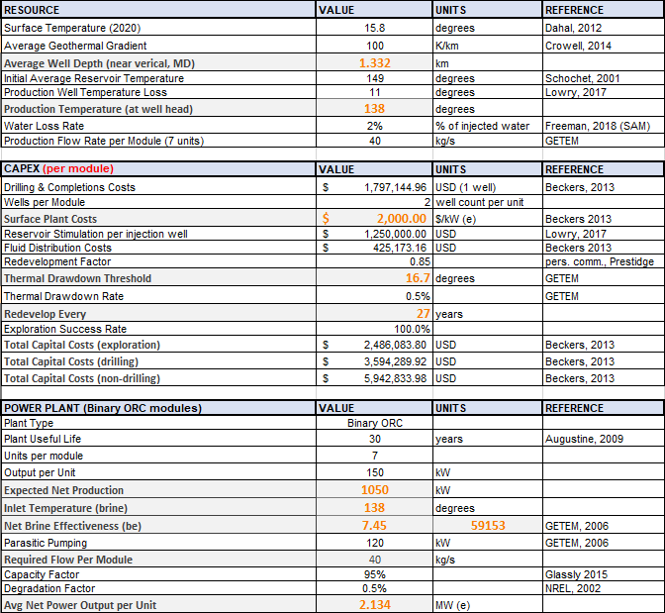
\includegraphics[width=\textwidth]{templates/images/Figure-Static_Model_SheetA.png}
\caption[Static cost model worksheet (part 1)]{First part of geothermal power plant expansion static NPV cost model.}
\label{fig:static_model_sheet1}
\end{figure}

\begin{figure}[H]
\centering
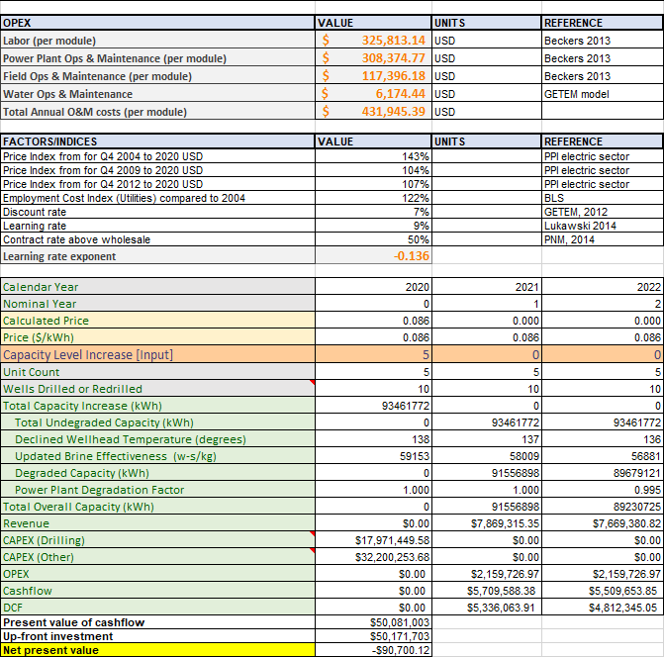
\includegraphics[width=\textwidth]{templates/images/Figure-Static_Model_SheetB.png}
\caption[Static cost model worksheet (part 2)]{Second part of geothermal power plant expansion static NPV cost model. The yearly breakdown of cost and revenue only extends out to year 2 for visualization purposes but continues to year 30 in the actual spreadsheet.}
\label{fig:static_model_sheet2}
\end{figure}
\pagebreak
\section{Flexible NPV Models}\label{app:B_flex_models}

\textbf{TO BE ADDED}
%% This defines the bibliography file (main.bib) and the bibliography style.
%% If you want to create a bibliography file by hand, change the contents of
%% this file to a `thebibliography' environment.  For more information 
%% see section 4.3 of the LaTeX manual.
\begin{singlespace}
\bibliography{main}

%% APA citation
\bibliographystyle{apacite}
\end{singlespace}

\end{document}
